\providecommand{\slides}{
  \newcommand{\slideshead}{
  \newcommand{\thepage}{\arabic{mypage}}
  %beamer
  \documentclass[t,hyperref={bookmarks=true}]{beamer}
%  \documentclass[t,hyperref={bookmarks=true},aspectratio=169]{beamer}
  \setbeamersize{text margin left=5mm}
  \setbeamersize{text margin right=5mm}
  \usetheme{default}
  \usefonttheme[onlymath]{serif}
  \setbeamertemplate{navigation symbols}{}
  \setbeamertemplate{itemize items}{{\color{black}$\bullet$}}

  \newwrite\keyfile

  %\usepackage{palatino}
  \stdpackages
  \usepackage{multimedia}

  %%% geometry/spacing issues
  %
  \definecolor{bluecol}{rgb}{0,0,.5}
  \definecolor{greencol}{rgb}{0,.6,0}
  %\renewcommand{\baselinestretch}{1.1}
  \renewcommand{\arraystretch}{1.2}
  \columnsep 0mm

  \columnseprule 0pt
  \parindent 0ex
  \parskip 0ex
  %\setlength{\itemparsep}{3ex}
  %\renewcommand{\labelitemi}{\rule[3pt]{10pt}{10pt}~}
  %\renewcommand{\labelenumi}{\textbf{(\arabic{enumi})}}
  \newcommand{\headerfont}{\helvetica{13}{1.5}{b}{n}}
  \newcommand{\slidefont} {\helvetica{10}{1.4}{m}{n}}
  \newcommand{\codefont} {\helvetica{8}{1.2}{m}{n}}
  \renewcommand{\small} {\helvetica{9}{1.4}{m}{n}}
  \renewcommand{\tiny} {\helvetica{8}{1.3}{m}{n}}
  \newcommand{\ttiny} {\helvetica{7}{1.3}{m}{n}}

  %%% count pages properly and put the page number in bottom right
  %
  \newcounter{mypage}
  \newcommand{\incpage}{\addtocounter{mypage}{1}\setcounter{page}{\arabic{mypage}}}
  \setcounter{mypage}{0}
  \resetcounteronoverlays{page}

  \pagestyle{fancy}
  %\setlength{\headsep}{10mm}
  %\addtolength{\footheight}{15mm}
  \renewcommand{\headrulewidth}{0pt} %1pt}
  \renewcommand{\footrulewidth}{0pt} %.5pt}
  \cfoot{}
  \rhead{}
  \lhead{}
%  \rfoot{{\tiny\textsf{AI -- \topic -- \subtopic -- \arabic{mypage}/\pageref{lastpage}}}}
%  \rfoot{\vspace*{-4.5mm}{\tiny\textsf{\topic\ -- \subtopic\ -- \arabic{mypage}/\pageref{lastpage}}}\hspace*{-4mm}}
  \rfoot{\vspace*{-4.5mm}{\tiny\textsf{\color{gray}\topic\ -- \subtopic\ -- \arabic{mypage}/\pageref{lastpage}}}\hspace*{-4mm}}
  %\lfoot{\raisebox{5mm}{\tiny\textsf{\slideauthor}}}
  %\rfoot{\raisebox{5mm}{\tiny\textsf{\slidevenue{} -- \arabic{mypage}/\pageref{lastpage}}}}
  %\rfoot{~\anchor{30,12}{\tiny\textsf{\thepage/\pageref{lastpage}}}}
  %\lfoot{\small\textsf{Marc Toussaint}}

  \definecolor{grey}{rgb}{.8,.8,.8}
  \definecolor{head}{rgb}{.85,.9,.9}
  \definecolor{blue}{rgb}{.0,.0,.5}
  \definecolor{green}{rgb}{.0,.5,.0}
  \definecolor{red}{rgb}{.8,.0,.0}
  \newcommand{\inverted}{
    \definecolor{main}{rgb}{1,1,1}
    \color{main}
    \pagecolor[rgb]{.3,.3,.3}
  }
  %auto-ignore
  \renewcommand{\a}{\alpha}
  \renewcommand{\b}{\beta}
  \renewcommand{\d}{\delta}
    \newcommand{\D}{\Delta}
    \newcommand{\e}{\epsilon}
    \newcommand{\g}{\gamma}
    \newcommand{\G}{\Gamma}
  \renewcommand{\l}{\lambda}
  \renewcommand{\L}{\Lambda}
    \newcommand{\m}{\mu}
    \newcommand{\n}{\nu}
    \newcommand{\N}{\nabla}
  \renewcommand{\k}{\kappa}
  \renewcommand{\o}{\omega}
  \renewcommand{\O}{\Omega}
    \newcommand{\p}{\phi}
    \newcommand{\ph}{\varphi}
  \renewcommand{\P}{\Phi}
  \renewcommand{\r}{\varrho}
    \newcommand{\s}{\sigma}
  \renewcommand{\S}{\Sigma}
  \renewcommand{\t}{\theta}
    \newcommand{\T}{\Theta}
  %\renewcommand{\v}{\vartheta}
    \newcommand{\x}{\xi}
    \newcommand{\X}{\Xi}
    \newcommand{\Y}{\Upsilon}
    \newcommand{\z}{\zeta}

  \renewcommand{\AA}{{\cal A}}
    \newcommand{\BB}{{\cal B}}
    \newcommand{\CC}{{\cal C}}
    \newcommand{\cc}{{\cal c}}
    \newcommand{\DD}{{\cal D}}
    \newcommand{\EE}{{\cal E}}
    \newcommand{\FF}{{\cal F}}
    \newcommand{\GG}{{\cal G}}
    \newcommand{\HH}{{\cal H}}
    \newcommand{\II}{{\cal I}}
    \newcommand{\KK}{{\cal K}}
    \newcommand{\LL}{{\cal L}}
    \newcommand{\MM}{{\cal M}}
    \newcommand{\NN}{{\cal N}}
    \newcommand{\oNN}{\overline\NN}
    \newcommand{\OO}{{\cal O}}
    \newcommand{\PP}{{\cal P}}
    \newcommand{\QQ}{{\cal Q}}
    \newcommand{\RR}{{\cal R}}
  \renewcommand{\SS}{{\cal S}}
    \newcommand{\TT}{{\cal T}}
    \newcommand{\uu}{{\cal u}}
    \newcommand{\UU}{{\cal U}}
    \newcommand{\VV}{{\cal V}}
    \newcommand{\XX}{{\cal X}}
    \newcommand{\xx}{\mathcal{x}}
    \newcommand{\YY}{{\cal Y}}
    \newcommand{\SOSO}{{\cal SO}}
    \newcommand{\GLGL}{{\cal GL}}

    \newcommand{\Ee}{{\rm E}}

  \newcommand{\NNN}{{\mathbb{N}}}
  \newcommand{\III}{{\mathbb{I}}}
  \newcommand{\ZZZ}{{\mathbb{Z}}}
  %\newcommand{\RRR}{{\mathrm{I\!R}}}
  \newcommand{\RRR}{{\mathbb{R}}}
  \newcommand{\SSS}{{\mathbb{S}}}
  \newcommand{\CCC}{{\mathbb{C}}}
  \newcommand{\DDD}{{\mathbb{D}}}
  \newcommand{\one}{{{\bf 1}}}
  \newcommand{\eee}{\text{e}}

  \newcommand{\NNNN}{{\overline{\cal N}}}

  \renewcommand{\[}{\Big[}
  \renewcommand{\]}{\Big]}
  \renewcommand{\(}{\Big(}
  \renewcommand{\)}{\Big)}
  \renewcommand{\|}{\,|\,}
  \renewcommand{\;}{\,;\,}
  \renewcommand{\=}{\!=\!}
    \newcommand{\<}{\left\langle}
  \renewcommand{\>}{\right\rangle}

  \newcommand{\na}[1][]{{\nabla_{\!\!#1}}}
  \newcommand{\he}[1][]{{\nabla_{\!\!#1}^2}}
  \newcommand{\Prob}{{\rm Prob}}
  \newcommand{\Dir}{{\rm Dir}}
  \newcommand{\Beta}{{\rm Beta}}
  \newcommand{\Bern}{{\rm Bern}}
  \newcommand{\Bin}{{\rm Bin}}
  \newcommand{\Mult}{{\rm Mult}}
  \newcommand{\Aut}{{\rm Aut}}
  \newcommand{\cor}{{\rm cor}}
  \newcommand{\corr}{{\rm corr}}
  \newcommand{\sd}{{\rm sd}}
  \newcommand{\tr}{{\rm tr}}
  \newcommand{\Tr}{{\rm Tr}}
  \newcommand{\rank}{{\rm rank}}
  \newcommand{\diag}{{\rm diag}}
  \newcommand{\dom}{{\rm dom}}
  \newcommand{\id}{{\rm id}}
  \newcommand{\Id}{{\rm\bf I}}
  \newcommand{\Gl}{{\rm Gl}}
  \renewcommand{\th}{\ensuremath{{}^\text{th}} }
  \newcommand{\lag}{\mathcal{L}}
  \newcommand{\inn}{\rfloor}
  \newcommand{\lie}{\pounds}
  \newcommand{\longto}{\longrightarrow}
  \newcommand{\speer}{\parbox{0.4ex}{\raisebox{0.8ex}{$\nearrow$}}}
  \renewcommand{\dag}{ {}^\dagger }
  \newcommand{\blbox}{\rule{1ex}{1ex}}
  \newcommand{\Ji}{J^\sharp}
  \newcommand{\h}{{}^\star}
  \newcommand{\w}{\wedge}
  \newcommand{\too}{\longrightarrow}
  \newcommand{\oot}{\longleftarrow}
  \newcommand{\To}{\Rightarrow}
  \newcommand{\oT}{\Leftarrow}
  \newcommand{\oTo}{\Leftrightarrow}
  \renewcommand{\iff}{~\Longleftrightarrow~}
  \newcommand{\Too}{\;\Longrightarrow\;}
  \newcommand{\oto}{\leftrightarrow}
  \newcommand{\ot}{\leftarrow}
  \newcommand{\ootoo}{\longleftrightarrow}
  \newcommand{\ow}{\stackrel{\circ}\wedge}
  \newcommand{\defeq}{\stackrel{\hspace{0.2ex}{}_\Delta}=}
%  \newcommand{\defeq}{{\overstack\Delta =}}
  \newcommand{\feed}{\nonumber \\}
  \newcommand{\comma}{~,\quad}
  \newcommand{\period}{~.\quad}
  \newcommand{\del}{\partial}
%  \newcommand{\quabla}{\Delta}
  \newcommand{\point}{$\bullet~~$}
  \newcommand{\doubletilde}{ ~ \raisebox{0.3ex}{$\widetilde {}$} \raisebox{0.6ex}{$\widetilde {}$} \!\! }
  \newcommand{\topcirc}{\parbox{0ex}{~\raisebox{2.5ex}{${}^\circ$}}}
  \newcommand{\topdot} {\parbox{0ex}{~\raisebox{2.5ex}{$\cdot$}}}
  \newcommand{\topddot} {\parbox{0ex}{~\raisebox{1.3ex}{$\ddot{~}$}}}
  \newcommand{\sym}{\topcirc}
  \newcommand{\tsum}{\textstyle\sum}
  \newcommand{\st}{\quad\text{s.t.}\quad}

  \newcommand{\half}{\ensuremath{\frac{1}{2}}}
  \newcommand{\third}{\ensuremath{\frac{1}{3}}}
  \newcommand{\fourth}{\ensuremath{\frac{1}{4}}}

  \newcommand{\ubar}{\underline}
  %\renewcommand{\vec}{\underline}
  \renewcommand{\vec}{\boldsymbol}
  %\renewcommand{\_}{\underset}
  %\renewcommand{\^}{\overset}
  %\renewcommand{\*}{{\rm\raisebox{-.6ex}{\text{*}}{}}}
  \renewcommand{\*}{\text{\footnotesize\raisebox{-.4ex}{*}{}}}

  \newcommand{\gto}{{\raisebox{.5ex}{${}_\rightarrow$}}}
  \newcommand{\gfrom}{{\raisebox{.5ex}{${}_\leftarrow$}}}
  \newcommand{\gnto}{{\raisebox{.5ex}{${}_\nrightarrow$}}}
  \newcommand{\gnfrom}{{\raisebox{.5ex}{${}_\nleftarrow$}}}

  %\newcommand{\RND}{{\SS}}
  %\newcommand{\IF}{\text{if }}
  %\newcommand{\AND}{\textsc{and }}
  %\newcommand{\OR}{\textsc{or }}
  %\newcommand{\XOR}{\textsc{xor }}
  %\newcommand{\NOT}{\textsc{not }}

  %\newcommand{\argmax}[1]{{\rm arg}\!\max_{#1}}
  %\newcommand{\argmin}[1]{{\rm arg}\!\min_{#1}}
  \DeclareMathOperator*{\argmax}{argmax}
  \DeclareMathOperator*{\argmin}{argmin}
  \DeclareMathOperator{\sign}{sign}
  \DeclareMathOperator{\acos}{acos}
  \DeclareMathOperator{\unifies}{unifies}
  \DeclareMathOperator{\Span}{span}
  \newcommand{\ortho}{\perp}
  %\newcommand{\argmax}[1]{\underset{~#1}{\text{argmax}}\;}
  %\newcommand{\argmin}[1]{\underset{~#1}{\text{argmin}}\;}
  \newcommand{\ee}[1]{\ensuremath{\cdot10^{#1}}}
  \newcommand{\sub}[1]{\ensuremath{_{\text{#1}}}}
  \newcommand{\up}[1]{\ensuremath{^{\text{#1}}}}
  \newcommand{\kld}[3][{}]{D_{#1}\big(#2\,\big|\!\big|\,#3\big)}
  %\newcommand{\kld}[2]{D\big(#1:#2\big)}
  \newcommand{\sprod}[2]{\big<#1\,,\,#2\big>}
  \newcommand{\End}{\text{End}}
  \newcommand{\txt}[1]{\quad\text{#1}\quad}
  \newcommand{\Over}[2]{\genfrac{}{}{0pt}{0}{#1}{#2}}
  %\newcommand{\mat}[1]{{\bf #1}}
  \newcommand{\arr}[2]{\hspace*{-.5ex}\begin{array}{#1}#2\end{array}\hspace*{-.5ex}}
  \newcommand{\mat}[3][.9]{
    \renewcommand{\arraystretch}{#1}{\scriptscriptstyle{\left(
      \hspace*{-1ex}\begin{array}{#2}#3\end{array}\hspace*{-1ex}
    \right)}}\renewcommand{\arraystretch}{1.2}
  }
  \newcommand{\Mat}[3][.9]{
    \renewcommand{\arraystretch}{#1}{\scriptscriptstyle{\left[
      \hspace*{-1ex}\begin{array}{#2}#3\end{array}\hspace*{-1ex}
    \right]}}\renewcommand{\arraystretch}{1.2}
  }
  \newcommand{\case}[2][ll]{\left\{\arr{#1}{#2}\right.}
  \newcommand{\seq}[1]{\textsf{\<#1\>}}
  \newcommand{\seqq}[1]{\textsf{#1}}
  \newcommand{\floor}[1]{\lfloor#1\rfloor}
  \newcommand{\Exp}[2][]{\text{E}_{#1}\{#2\}}
  \newcommand{\Var}[2][]{\text{Var}_{#1}\{#2\}}
  \newcommand{\cov}[2][]{\text{cov}_{#1}\{#2\}}

  %\newcommand{\Exp}[2]{\left\langle{#2}\right\rangle_{#1}}
  \newcommand{\ex}{\setminus}

  \providecommand{\href}[2]{{\color{blue}USE PDFLATEX!}}
  \providecommand{\url}[2]{\href{#1}{{\color{blue}#2}}}
%  \newcommand{\link}[1]{\href{{\protect #1}}{\texttt{\protect #1}}}
  \newcommand{\anchor}[2]{\begin{picture}(0,0)\put(#1){#2}\end{picture}}
  \newcommand{\pagebox}{\begin{picture}(0,0)\put(-3,-23){
    \textcolor[rgb]{.5,1,.5}{\framebox[\textwidth]{\rule[-\textheight]{0pt}{0pt}}}}
    \end{picture}}

  \newcommand{\hide}[1]{
    \begin{list}{}{\leftmargin0ex \rightmargin0ex \topsep0ex \parsep0ex}
       \helvetica{5}{1}{m}{n}
       \renewcommand{\section}{\par SECTION: }
       \renewcommand{\subsection}{\par SUBSECTION: }
       \item[$~~\blacktriangleright$]
       #1%$\blacktriangleleft~~$
       \message{^^JHIDE--Warning!^^J}
    \end{list}
  }
  %\newcommand{\hide}[1]{{\tt[hide:~}{\footnotesize\sf #1}{\tt]}\message{^^JHIDE--Warning!^^J}}
  \newcommand{\Hide}{\renewcommand{\hide}[1]{\message{^^JHIDE--Warning (hidden)!^^J}}}
  \newcommand{\HIDE}{\renewcommand{\hide}[1]{}}
  \newcommand{\fullhide}[1]{\message{^^JHIDE--Warning (hidden)!^^J}}
  \newcommand{\todo}[1]{{\tt[TODO: #1]}\message{^^JTODO--Warning: #1^^J}}
  \newcommand{\Todo}{\renewcommand{\todo}[1]{\message{^^JTODO--Warning (hidden)!^^J}}}
  %\renewcommand{\title}[1]{\renewcommand{\thetitle}{#1}}
  \newcommand{\myauthor}[1]{\author{#1}\newcommand{\theauthor}{#1}}%\@author}
  \newcommand{\mytitle}[1]{\title{#1}\newcommand{\thetitle}{#1}}%\@title}
  \newcommand{\header}{\begin{document}\mytitle\cleardefs}
  \newcommand{\contents}{{\tableofcontents}\renewcommand{\contents}{}}
  \newcommand{\footer}{\small\bibliography{marc,bibs}\end{document}}
  \newcommand{\widepaper}{\usepackage{geometry}\geometry{a4paper,hdivide={25mm,*,25mm},vdivide={25mm,*,25mm}}}
  \newcommand{\moviex}[2]{\movie[externalviewer]{#1}{#2}} %\pdflatex\usepackage{multimedia}
  \newcommand{\rbox}[1]{\fboxrule2mm\fcolorbox[rgb]{1,.85,.85}{1,.85,.85}{#1}}
  \newcommand{\mpage}[2]{{\begin{minipage}{#1\columnwidth}#2\end{minipage}}}
  \newcommand{\redbox}[2]{\fboxrule1mm\fcolorbox[rgb]{1,.7,.7}{1,.7,.7}{\begin{minipage}{#1\columnwidth}\center#2\end{minipage}}}
  \newcommand{\onecol}[2]{
    \begin{minipage}[c]{#1\columnwidth}#2\end{minipage}}
  \newcommand{\twocol}[5][0]{
    \begin{minipage}[c]{#2\columnwidth}#4\end{minipage}\hspace*{#1\columnwidth}%
    \begin{minipage}[c]{#3\columnwidth}#5\end{minipage}}
  \newcommand{\threecol}[7][0]{%
    \begin{minipage}[c]{#2\columnwidth}#5\end{minipage}\hspace*{#1\columnwidth}%
    \begin{minipage}[c]{#3\columnwidth}#6\end{minipage}\hspace*{#1\columnwidth}%
    \begin{minipage}[c]{#4\columnwidth}#7\end{minipage}}
  \newcommand{\threecoltext}[7][c]{
    \begin{minipage}[#1]{#2\textwidth}#5\end{minipage}%
    \begin{minipage}[#1]{#3\textwidth}#6\end{minipage}%
    \begin{minipage}[#1]{#4\textwidth}#7\end{minipage}}
  \newcommand{\threecoltop}[7][0]{%
   \begin{minipage}[t]{#2\columnwidth}#5\end{minipage}\hspace*{#1\columnwidth}%
   \begin{minipage}[t]{#3\columnwidth}#6\end{minipage}\hspace*{#1\columnwidth}%
   \begin{minipage}[t]{#4\columnwidth}#7\end{minipage}}
  \newcommand{\fourcol}[9][0]{%
   \begin{minipage}[c]{#2\columnwidth}#6\end{minipage}\hspace*{#1\columnwidth}%
   \begin{minipage}[c]{#3\columnwidth}#7\end{minipage}\hspace*{#1\columnwidth}%
   \begin{minipage}[c]{#4\columnwidth}#8\end{minipage}\hspace*{#1\columnwidth}%
   \begin{minipage}[c]{#5\columnwidth}#9\end{minipage}}
  \newcommand{\helvetica}[4]{\setlength{\unitlength}{1pt}\fontsize{#1}{#1}\linespread{#2}\usefont{OT1}{phv}{#3}{#4}}
  \newcommand{\helve}[1]{\helvetica{#1}{1.5}{m}{n}}
  \newcommand{\german}{\usepackage[german]{babel}\usepackage[utf8]{inputenc}}

\newcommand{\norm}[1]{|\!|#1|\!|}
\newcommand{\expr}[1]{[\hspace{-.2ex}[#1]\hspace{-.2ex}]}

\newcommand{\Jwi}{J^\sharp_W}
\newcommand{\THi}{T^\sharp_H}
\newcommand{\Jci}{J^\natural_C}
\newcommand{\hJi}{{\bar J}^\sharp}
\renewcommand{\|}{\,|\,}
\renewcommand{\=}{\!=\!}
\newcommand{\myminus}{{\hspace*{-.0pt}\text{\rm -}\hspace*{-.5pt}}}
\newcommand{\myplus}{{\hspace*{-.0pt}\text{\rm +}\hspace*{-.5pt}}}
\newcommand{\1}{{\myminus1}}
\newcommand{\2}{{\myminus2}}
\newcommand{\3}{{\myminus3}}
\newcommand{\mT}{{\text{\rm -}\hspace*{-1pt}\top}}
\newcommand{\po}{{\myplus1}}
\newcommand{\pt}{{\myplus2}}
%\renewcommand{\-}{\myminus}
%\newcommand{\+}{\myplus}
\renewcommand{\T}{{\!\top\!}}
\newcommand{\xT}{{\underline x}}
\newcommand{\uT}{{\underline u}}
\newcommand{\zT}{{\underline z}}
\newcommand{\Sum}{\textstyle\sum}
\newcommand{\Int}{\textstyle\int}
\newcommand{\Prod}{\textstyle\prod}


\newenvironment{centy}{
\vspace{15mm}
\large
\hspace*{5mm}
\begin{minipage}{8cm}\it\color{blue}
}{
\end{minipage}
}

\newcommand{\old}{{\text{old}}}
\newcommand{\new}{{\text{new}}}
\newcommand{\MAP}{{\text{MAP}}}
\newcommand{\ML}{{\text{ML}}}

\newcommand{\redArrow}{\quad\anchor{0,-1}{\includegraphics[scale=.5]{figs/redArrow}}}
\newcommand{\pub}[1]{{\color{green}\helvetica{8}{1.3}{m}{n}#1\\}}
\DeclareMathOperator{\opKL}{KL}
\newcommand{\KL}[2]{\opKL\big(#1\,\big|\!\big|\,#2\big)} %\left(#1 |\!| #2\right)}

\renewcommand{\show}[2][.8]{\centerline{\includegraphics[width=#1\columnwidth]{#2}}}
\newcommand{\showh}[2][.8]{\includegraphics[width=#1\columnwidth]{#2}}
\newcommand{\shows}[2][.8]{\centerline{\includegraphics[scale=#1]{#2}}}
\newcommand{\showhs}[2][.8]{\includegraphics[scale=#1]{#2}}
\newcommand{\mov}[2]{\movie[externalviewer]{{\color{blue}\small #1}}{movies/#2}}
\newcommand{\movex}[2]{\movie[externalviewer]{#1}{#2}} %\pdflatex\usepackage{multimedia}
%\newcommand{\movgb}[1]{\hfill\movie[externalviewer]{\small[movie]}{/home/mtoussai/movies/10-goalDirectedBehavior/#1}}
\newcommand{\movh}[3][loop]{
\movie[#1]{\showh[#2]{movies/#3.png}}{movies/#3.avi}%
\movie[externalviewer]{$\circ$}{movies/#3.avi}
}
\newcommand{\movc}[3][loop]{\centerline{\movh[#1]{#2}{#3}}}
\newcommand{\cen}[1]{\centerline{#1}}

\newcommand{\citing}[1]{
{\color{citcol}\tiny#1\par}
}

\newcommand{\cit}[3]{
\par\smallskip
{\color{greencol}\tiny #1: \emph{#2}. #3 \par}
}

\newcommand{\citurl}[4]{
\par\smallskip
{\color{greencol}\tiny #1: \protect{\href{#4}{\color{blue}{#2.}}} #3 \par}
}

\newcommand{\cito}[3]{
\par\smallskip
{\color{bluecol}\tiny #1: \emph{#2}. #3 \par}
}

\newcommand{\redoMacrosInProof}{
  \renewcommand{\d}{\delta}
%  \renewcommand{\|}{\,|\,}
  \renewcommand{\=}{\!=\!}
}

%% \makeatletter
%% \newenvironment{code}{%
%%   \begin{lrbox}{\@tempboxa}\begin{minipage}{1\columnwidth}\codefont
%% }{
%%   \end{minipage}\end{lrbox}%
%%   \colorbox[rgb]{.95,.95,.95}{\usebox{\@tempboxa}}
%% }\makeatother

\newenvironment{code}{%
\codefont
\begin{shaded}
}{
\end{shaded}
}

%\newcommand{\refeq}[1]{(\ref{#1})}

\usepackage{algorithm}
\usepackage{algpseudocode}
\algrenewcommand{\algorithmicrequire}{\textbf{Input:~~}}
\algrenewcommand{\algorithmicensure}{\textbf{Output:}}
\algrenewcommand{\algorithmiccomment}[1]{\qquad\hfill~\hspace*{-5ex}\textit{// #1}}
\algrenewcommand{\alglinenumber}[1]{\helvetica{6}{1.3}{m}{n}#1:}

\newenvironment{algo}[1][8]{
\quad\begin{minipage}{.8\columnwidth}\helvetica{#1}{1.3}{m}{n}
\medskip\hrule\medskip
\begin{algorithmic}[1]
}{
\end{algorithmic}
\medskip\hrule\medskip
\end{minipage}
}

\usepackage{etoolbox}

%%%%%%%%%%%%%%%%%%%%%%%%%%%%%%%%%%%%%%%%%%%%%%%%%%%%%%%%%%%%%%%%%%%%%%%%%%%%%%%%

\usepackage{multirow}
\usepackage{colortbl}
%\setlength{\jot}{0pt}
%\setlength{\mathindent}{1ex}
\usepackage{empheq}

%%%%%%%%%%%%%%%%%%%%%%%%%%%%%%%%%%%%%%%%%%%%%%%%%%%%%%%%%%%%%%%%%%%%%%%%%%%%%%%

\newcommand{\mypause}{\pause}
%\newcommand{\dom}{{\text{dom}}}
\newcommand{\defi}[1]{\textbf{#1}}
\newcommand{\red}[1]{\emph{\color{red}#1}}
%\newcommand{\ul}{\underline}
\newcommand{\pos}{{\textsf{pos}}}
\newcommand{\eff}{{\textsf{eff}}}
\newcommand{\rot}{{\textsf{rot}}}
\newcommand{\veC}{{\textsf{vec}}}
\newcommand{\quat}{{\textsf{quat}}}
\newcommand{\col}{{\textsf{col}}}
\newcommand{\de}[2]{\frac{\partial #1}{\partial #2}}
\newcommand{\target}{{\text{target}}}
\newcommand{\near}{{\text{near}}}
\newcommand{\qfree}{Q_{\text{free}}}
\renewcommand{\vec}{\boldsymbol}
\newcommand{\lft}{\text{left}}
\newcommand{\rgh}{\text{right}}
\DeclareMathOperator{\real}{real}
\newcommand{\prev}{{\text{prev}}}
\newcommand{\TR}[2]{T_{{#1}\shortrightarrow{#2}}}
\newcommand{\RO}[2]{R_{{#1}\shortrightarrow{#2}}}
\newcommand{\liter}{\helvetica{8}{1.1}{m}{n}\parskip 1ex}
\newcommand{\Fc}{\color{green}F}
\newcommand{\muc}{\color{blue}\mu}
\newcommand{\Astar}{A$^*$}

%for optimization course:
\newcommand{\adec}{\r_\a^-}
\newcommand{\ainc}{\r_\a^+}
\newcommand{\ldec}{\r_\l^-}
\newcommand{\linc}{\r_\l^+}
\newcommand{\minc}{\r_\m^+}
\newcommand{\mdec}{\r_\m^-}
\newcommand{\lsstop}{\r_{\text{ls}}}


\definecolor{boxcol}{rgb}{.85,.9,.92}
\newcommand{\eqbox}[1]{\centerline{\fboxrule0mm\fcolorbox{boxcol}{boxcol}{#1}}}
\newcommand{\movgb}[1]{\hfill\movie[externalviewer]{\small[movie]}{/home/mtoussai/movies/10-goalDirectedBehavior/#1}}
\newcommand{\demo}[1]{{{\color{blue}[\small #1]}}}

\graphicspath{{../pics-robotics/}{../pics-ML/}{../pics-all/}{../pics-all2/}{../pics-Optim/}}
\DeclareGraphicsExtensions{.pdf,.png,.jpg}

%\usepackage{pdfpages}
%\setbeamercolor{background canvas}{bg=}

\newcommand{\SUM}{\texttt{sum}}
\usepackage{float}

%% prevent pagebreaks before environment
\makeatletter
\newcommand{\NewParNoBreak}[1][\parskip]{\par\vspace*{-\parskip}\vspace*{#1}\nobreak\@afterheading}
\makeatother

%\newcommand{\idx}[2]{\label{IKgn}}

%%%%%%%%%%%%%%%%%%%%%%%%%%%%%%%%%%%%%%%%%%%%%%%%%%%%%%%%%%%%%%%%%%%%%%%%%%%%%%%%



%% \newwrite\tempfile
%% \immediate\openout\tempfile=z.keys.tex

%% \renewcommand{\key}[1]{
%% %%   \addtocounter{mypage}{1}
%% \makeatletter
%% \immediate\write\tempfile{\symbol{`\\}}
%% \makeatother
%%   \immediate\write\tempfile{hyperref[key:#1]{#1(\arabic{mypage})}}
%% %%  % \phantomsection\label{key:#1}
%% %%   %\index{#1@{\hyperref[key:#1]{#1 (\arabic{mysec}:\arabic{mypage})}}|phantom}
%% %%   \addtocounter{mypage}{-1}
%% }


  \graphicspath{{pics/}{../shared/pics/}}

  \title{Machine Learning \topic}
  \author{Marc Toussaint}
  \institute{Machine Learning \& Robotics Lab, U Stuttgart}

  \begin{document}

  \rfoot{\vspace*{-5mm}{\tiny
  \textsf{\arabic{mypage}/\pageref{lastpage}}}\hspace*{-4mm}}

  %% title slide!
  \slide{}{
    \thispagestyle{empty}

    \twocol{.27}{.6}{
      \hspace*{-15mm}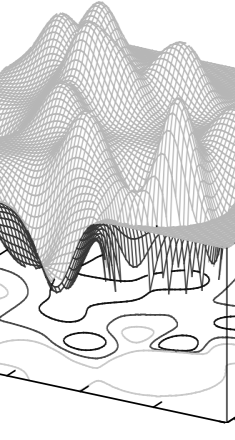
\includegraphics[height=7cm]{classPicture2-bw}
    }{\center

      \textbf{\fontsize{17}{20}\selectfont \course}

      ~

      %Lecture
      \topic\\

      \vspace{1cm}

      {\tiny~\emph{\keywords}~\\}

      \vspace{1cm}

      Marc Toussaint
      
      University of Stuttgart

      Summer 2019

      ~

    }
  }
}

\newcommand{\slide}[2]{
  \slidefont
  \incpage\begin{frame}
  \addcontentsline{toc}{section}{#1}
  \vfill
  {\headerfont #1} \vspace*{-2ex}
  \begin{itemize}\item[]~\\
    #2
  \end{itemize}
  \vfill
  \end{frame}
}

\newenvironment{slidecore}[1]{
  \slidefont\incpage
  \addcontentsline{toc}{section}{#1}
  \vfill
  {\headerfont #1} \vspace*{-2ex}
  \begin{itemize}\item[]~\\
}{
  \end{itemize}
  \vfill
}


\providecommand{\key}[1]{
  \addtocounter{mypage}{1}
% \immediate\write\keyfile{#1}
  \addtocontents{toc}{\hyperref[key:#1]{#1 (\arabic{mypage})}}
%  \phantomsection\label{key:#1}
%  \index{#1@{\hyperref[key:#1]{#1 (\arabic{mysec}:\arabic{mypage})}}|phantom}
  \addtocounter{mypage}{-1}
}

\providecommand{\course}{}

\providecommand{\subtopic}{}

\providecommand{\sublecture}[2]{
  \renewcommand{\subtopic}{#1}
  \slide{#1}{#2}
}

\providecommand{\story}[1]{
~

Motivation: {\tiny #1}\clearpage
}

\newenvironment{items}[1][9]{
\par\setlength{\unitlength}{1pt}\fontsize{#1}{#1}\linespread{1.2}\selectfont
\begin{list}{--}{\leftmargin4ex \rightmargin0ex \labelsep1ex \labelwidth2ex
\topsep0pt \parsep0ex \itemsep3pt}
}{
\end{list}
}

\providecommand{\slidesfoot}{
  \end{document}
}


  \slideshead
}

\providecommand{\exercises}{
  \newcommand{\exerciseshead}{
  \documentclass[10pt,fleqn]{article}
  \stdpackages

  \definecolor{bluecol}{rgb}{0,0,.5}
  \definecolor{greencol}{rgb}{0,.4,0}
  \definecolor{shadecolor}{gray}{0.9}
  \usepackage[
    %    pdftex%,
    %%    letterpaper,
    %    bookmarks,
    %    bookmarksnumbered,
    colorlinks,
    urlcolor=bluecol,
    citecolor=black,
    linkcolor=bluecol,
    %    pagecolor=bluecol,
    pdfborder={0 0 0},
    %pdfborderstyle={/S/U/W 1},
    %%    backref,     %link from bibliography back to sections
    %%    pagebackref, %link from bibliography back to pages
    %%    pdfstartview=FitH, %fitwidth instead of fit window
    pdfpagemode=UseNone, %UseOutlines, %bookmarks are displayed by acrobat
    pdftitle={\course},
    pdfauthor={Marc Toussaint},
    pdfkeywords={}
  ]{hyperref}
  \DeclareGraphicsExtensions{.pdf,.png,.jpg,.eps}

  \renewcommand{\r}{\varrho}
  \renewcommand{\l}{\lambda}
  \renewcommand{\L}{\Lambda}
  \renewcommand{\b}{\beta}
  \renewcommand{\d}{\delta}
  \renewcommand{\k}{\kappa}
  \renewcommand{\t}{\theta}
  \renewcommand{\O}{\Omega}
  \renewcommand{\o}{\omega}
  \renewcommand{\SS}{{\cal S}}
  \renewcommand{\=}{\!=\!}
  %\renewcommand{\boldsymbol}{}
  %\renewcommand{\Chapter}{\chapter}
  %\renewcommand{\Subsection}{\subsection}

  \renewcommand{\baselinestretch}{1.1}
  \geometry{a4paper,headsep=7mm,hdivide={15mm,*,15mm},vdivide={20mm,*,15mm}}

  \fancyhead[L]{\thetitle, \textit{Marc Toussaint}---\today}
  \fancyhead[R]{\thepage}
  \fancyhead[C]{}
  \fancyfoot{}
  \pagestyle{fancy}

  \parindent 0pt
  \parskip 0.5ex

  \newcommand{\codefont}{\helvetica{8}{1.2}{m}{n}}

  %auto-ignore
  \renewcommand{\a}{\alpha}
  \renewcommand{\b}{\beta}
  \renewcommand{\d}{\delta}
    \newcommand{\D}{\Delta}
    \newcommand{\e}{\epsilon}
    \newcommand{\g}{\gamma}
    \newcommand{\G}{\Gamma}
  \renewcommand{\l}{\lambda}
  \renewcommand{\L}{\Lambda}
    \newcommand{\m}{\mu}
    \newcommand{\n}{\nu}
    \newcommand{\N}{\nabla}
  \renewcommand{\k}{\kappa}
  \renewcommand{\o}{\omega}
  \renewcommand{\O}{\Omega}
    \newcommand{\p}{\phi}
    \newcommand{\ph}{\varphi}
  \renewcommand{\P}{\Phi}
  \renewcommand{\r}{\varrho}
    \newcommand{\s}{\sigma}
  \renewcommand{\S}{\Sigma}
  \renewcommand{\t}{\theta}
    \newcommand{\T}{\Theta}
  %\renewcommand{\v}{\vartheta}
    \newcommand{\x}{\xi}
    \newcommand{\X}{\Xi}
    \newcommand{\Y}{\Upsilon}
    \newcommand{\z}{\zeta}

  \renewcommand{\AA}{{\cal A}}
    \newcommand{\BB}{{\cal B}}
    \newcommand{\CC}{{\cal C}}
    \newcommand{\cc}{{\cal c}}
    \newcommand{\DD}{{\cal D}}
    \newcommand{\EE}{{\cal E}}
    \newcommand{\FF}{{\cal F}}
    \newcommand{\GG}{{\cal G}}
    \newcommand{\HH}{{\cal H}}
    \newcommand{\II}{{\cal I}}
    \newcommand{\KK}{{\cal K}}
    \newcommand{\LL}{{\cal L}}
    \newcommand{\MM}{{\cal M}}
    \newcommand{\NN}{{\cal N}}
    \newcommand{\oNN}{\overline\NN}
    \newcommand{\OO}{{\cal O}}
    \newcommand{\PP}{{\cal P}}
    \newcommand{\QQ}{{\cal Q}}
    \newcommand{\RR}{{\cal R}}
  \renewcommand{\SS}{{\cal S}}
    \newcommand{\TT}{{\cal T}}
    \newcommand{\uu}{{\cal u}}
    \newcommand{\UU}{{\cal U}}
    \newcommand{\VV}{{\cal V}}
    \newcommand{\XX}{{\cal X}}
    \newcommand{\xx}{\mathcal{x}}
    \newcommand{\YY}{{\cal Y}}
    \newcommand{\SOSO}{{\cal SO}}
    \newcommand{\GLGL}{{\cal GL}}

    \newcommand{\Ee}{{\rm E}}

  \newcommand{\NNN}{{\mathbb{N}}}
  \newcommand{\III}{{\mathbb{I}}}
  \newcommand{\ZZZ}{{\mathbb{Z}}}
  %\newcommand{\RRR}{{\mathrm{I\!R}}}
  \newcommand{\RRR}{{\mathbb{R}}}
  \newcommand{\SSS}{{\mathbb{S}}}
  \newcommand{\CCC}{{\mathbb{C}}}
  \newcommand{\DDD}{{\mathbb{D}}}
  \newcommand{\one}{{{\bf 1}}}
  \newcommand{\eee}{\text{e}}

  \newcommand{\NNNN}{{\overline{\cal N}}}

  \renewcommand{\[}{\Big[}
  \renewcommand{\]}{\Big]}
  \renewcommand{\(}{\Big(}
  \renewcommand{\)}{\Big)}
  \renewcommand{\|}{\,|\,}
  \renewcommand{\;}{\,;\,}
  \renewcommand{\=}{\!=\!}
    \newcommand{\<}{\left\langle}
  \renewcommand{\>}{\right\rangle}

  \newcommand{\na}[1][]{{\nabla_{\!\!#1}}}
  \newcommand{\he}[1][]{{\nabla_{\!\!#1}^2}}
  \newcommand{\Prob}{{\rm Prob}}
  \newcommand{\Dir}{{\rm Dir}}
  \newcommand{\Beta}{{\rm Beta}}
  \newcommand{\Bern}{{\rm Bern}}
  \newcommand{\Bin}{{\rm Bin}}
  \newcommand{\Mult}{{\rm Mult}}
  \newcommand{\Aut}{{\rm Aut}}
  \newcommand{\cor}{{\rm cor}}
  \newcommand{\corr}{{\rm corr}}
  \newcommand{\sd}{{\rm sd}}
  \newcommand{\tr}{{\rm tr}}
  \newcommand{\Tr}{{\rm Tr}}
  \newcommand{\rank}{{\rm rank}}
  \newcommand{\diag}{{\rm diag}}
  \newcommand{\dom}{{\rm dom}}
  \newcommand{\id}{{\rm id}}
  \newcommand{\Id}{{\rm\bf I}}
  \newcommand{\Gl}{{\rm Gl}}
  \renewcommand{\th}{\ensuremath{{}^\text{th}} }
  \newcommand{\lag}{\mathcal{L}}
  \newcommand{\inn}{\rfloor}
  \newcommand{\lie}{\pounds}
  \newcommand{\longto}{\longrightarrow}
  \newcommand{\speer}{\parbox{0.4ex}{\raisebox{0.8ex}{$\nearrow$}}}
  \renewcommand{\dag}{ {}^\dagger }
  \newcommand{\blbox}{\rule{1ex}{1ex}}
  \newcommand{\Ji}{J^\sharp}
  \newcommand{\h}{{}^\star}
  \newcommand{\w}{\wedge}
  \newcommand{\too}{\longrightarrow}
  \newcommand{\oot}{\longleftarrow}
  \newcommand{\To}{\Rightarrow}
  \newcommand{\oT}{\Leftarrow}
  \newcommand{\oTo}{\Leftrightarrow}
  \renewcommand{\iff}{~\Longleftrightarrow~}
  \newcommand{\Too}{\;\Longrightarrow\;}
  \newcommand{\oto}{\leftrightarrow}
  \newcommand{\ot}{\leftarrow}
  \newcommand{\ootoo}{\longleftrightarrow}
  \newcommand{\ow}{\stackrel{\circ}\wedge}
  \newcommand{\defeq}{\stackrel{\hspace{0.2ex}{}_\Delta}=}
%  \newcommand{\defeq}{{\overstack\Delta =}}
  \newcommand{\feed}{\nonumber \\}
  \newcommand{\comma}{~,\quad}
  \newcommand{\period}{~.\quad}
  \newcommand{\del}{\partial}
%  \newcommand{\quabla}{\Delta}
  \newcommand{\point}{$\bullet~~$}
  \newcommand{\doubletilde}{ ~ \raisebox{0.3ex}{$\widetilde {}$} \raisebox{0.6ex}{$\widetilde {}$} \!\! }
  \newcommand{\topcirc}{\parbox{0ex}{~\raisebox{2.5ex}{${}^\circ$}}}
  \newcommand{\topdot} {\parbox{0ex}{~\raisebox{2.5ex}{$\cdot$}}}
  \newcommand{\topddot} {\parbox{0ex}{~\raisebox{1.3ex}{$\ddot{~}$}}}
  \newcommand{\sym}{\topcirc}
  \newcommand{\tsum}{\textstyle\sum}
  \newcommand{\st}{\quad\text{s.t.}\quad}

  \newcommand{\half}{\ensuremath{\frac{1}{2}}}
  \newcommand{\third}{\ensuremath{\frac{1}{3}}}
  \newcommand{\fourth}{\ensuremath{\frac{1}{4}}}

  \newcommand{\ubar}{\underline}
  %\renewcommand{\vec}{\underline}
  \renewcommand{\vec}{\boldsymbol}
  %\renewcommand{\_}{\underset}
  %\renewcommand{\^}{\overset}
  %\renewcommand{\*}{{\rm\raisebox{-.6ex}{\text{*}}{}}}
  \renewcommand{\*}{\text{\footnotesize\raisebox{-.4ex}{*}{}}}

  \newcommand{\gto}{{\raisebox{.5ex}{${}_\rightarrow$}}}
  \newcommand{\gfrom}{{\raisebox{.5ex}{${}_\leftarrow$}}}
  \newcommand{\gnto}{{\raisebox{.5ex}{${}_\nrightarrow$}}}
  \newcommand{\gnfrom}{{\raisebox{.5ex}{${}_\nleftarrow$}}}

  %\newcommand{\RND}{{\SS}}
  %\newcommand{\IF}{\text{if }}
  %\newcommand{\AND}{\textsc{and }}
  %\newcommand{\OR}{\textsc{or }}
  %\newcommand{\XOR}{\textsc{xor }}
  %\newcommand{\NOT}{\textsc{not }}

  %\newcommand{\argmax}[1]{{\rm arg}\!\max_{#1}}
  %\newcommand{\argmin}[1]{{\rm arg}\!\min_{#1}}
  \DeclareMathOperator*{\argmax}{argmax}
  \DeclareMathOperator*{\argmin}{argmin}
  \DeclareMathOperator{\sign}{sign}
  \DeclareMathOperator{\acos}{acos}
  \DeclareMathOperator{\unifies}{unifies}
  \DeclareMathOperator{\Span}{span}
  \newcommand{\ortho}{\perp}
  %\newcommand{\argmax}[1]{\underset{~#1}{\text{argmax}}\;}
  %\newcommand{\argmin}[1]{\underset{~#1}{\text{argmin}}\;}
  \newcommand{\ee}[1]{\ensuremath{\cdot10^{#1}}}
  \newcommand{\sub}[1]{\ensuremath{_{\text{#1}}}}
  \newcommand{\up}[1]{\ensuremath{^{\text{#1}}}}
  \newcommand{\kld}[3][{}]{D_{#1}\big(#2\,\big|\!\big|\,#3\big)}
  %\newcommand{\kld}[2]{D\big(#1:#2\big)}
  \newcommand{\sprod}[2]{\big<#1\,,\,#2\big>}
  \newcommand{\End}{\text{End}}
  \newcommand{\txt}[1]{\quad\text{#1}\quad}
  \newcommand{\Over}[2]{\genfrac{}{}{0pt}{0}{#1}{#2}}
  %\newcommand{\mat}[1]{{\bf #1}}
  \newcommand{\arr}[2]{\hspace*{-.5ex}\begin{array}{#1}#2\end{array}\hspace*{-.5ex}}
  \newcommand{\mat}[3][.9]{
    \renewcommand{\arraystretch}{#1}{\scriptscriptstyle{\left(
      \hspace*{-1ex}\begin{array}{#2}#3\end{array}\hspace*{-1ex}
    \right)}}\renewcommand{\arraystretch}{1.2}
  }
  \newcommand{\Mat}[3][.9]{
    \renewcommand{\arraystretch}{#1}{\scriptscriptstyle{\left[
      \hspace*{-1ex}\begin{array}{#2}#3\end{array}\hspace*{-1ex}
    \right]}}\renewcommand{\arraystretch}{1.2}
  }
  \newcommand{\case}[2][ll]{\left\{\arr{#1}{#2}\right.}
  \newcommand{\seq}[1]{\textsf{\<#1\>}}
  \newcommand{\seqq}[1]{\textsf{#1}}
  \newcommand{\floor}[1]{\lfloor#1\rfloor}
  \newcommand{\Exp}[2][]{\text{E}_{#1}\{#2\}}
  \newcommand{\Var}[2][]{\text{Var}_{#1}\{#2\}}
  \newcommand{\cov}[2][]{\text{cov}_{#1}\{#2\}}

  %\newcommand{\Exp}[2]{\left\langle{#2}\right\rangle_{#1}}
  \newcommand{\ex}{\setminus}

  \providecommand{\href}[2]{{\color{blue}USE PDFLATEX!}}
  \providecommand{\url}[2]{\href{#1}{{\color{blue}#2}}}
%  \newcommand{\link}[1]{\href{{\protect #1}}{\texttt{\protect #1}}}
  \newcommand{\anchor}[2]{\begin{picture}(0,0)\put(#1){#2}\end{picture}}
  \newcommand{\pagebox}{\begin{picture}(0,0)\put(-3,-23){
    \textcolor[rgb]{.5,1,.5}{\framebox[\textwidth]{\rule[-\textheight]{0pt}{0pt}}}}
    \end{picture}}

  \newcommand{\hide}[1]{
    \begin{list}{}{\leftmargin0ex \rightmargin0ex \topsep0ex \parsep0ex}
       \helvetica{5}{1}{m}{n}
       \renewcommand{\section}{\par SECTION: }
       \renewcommand{\subsection}{\par SUBSECTION: }
       \item[$~~\blacktriangleright$]
       #1%$\blacktriangleleft~~$
       \message{^^JHIDE--Warning!^^J}
    \end{list}
  }
  %\newcommand{\hide}[1]{{\tt[hide:~}{\footnotesize\sf #1}{\tt]}\message{^^JHIDE--Warning!^^J}}
  \newcommand{\Hide}{\renewcommand{\hide}[1]{\message{^^JHIDE--Warning (hidden)!^^J}}}
  \newcommand{\HIDE}{\renewcommand{\hide}[1]{}}
  \newcommand{\fullhide}[1]{\message{^^JHIDE--Warning (hidden)!^^J}}
  \newcommand{\todo}[1]{{\tt[TODO: #1]}\message{^^JTODO--Warning: #1^^J}}
  \newcommand{\Todo}{\renewcommand{\todo}[1]{\message{^^JTODO--Warning (hidden)!^^J}}}
  %\renewcommand{\title}[1]{\renewcommand{\thetitle}{#1}}
  \newcommand{\myauthor}[1]{\author{#1}\newcommand{\theauthor}{#1}}%\@author}
  \newcommand{\mytitle}[1]{\title{#1}\newcommand{\thetitle}{#1}}%\@title}
  \newcommand{\header}{\begin{document}\mytitle\cleardefs}
  \newcommand{\contents}{{\tableofcontents}\renewcommand{\contents}{}}
  \newcommand{\footer}{\small\bibliography{marc,bibs}\end{document}}
  \newcommand{\widepaper}{\usepackage{geometry}\geometry{a4paper,hdivide={25mm,*,25mm},vdivide={25mm,*,25mm}}}
  \newcommand{\moviex}[2]{\movie[externalviewer]{#1}{#2}} %\pdflatex\usepackage{multimedia}
  \newcommand{\rbox}[1]{\fboxrule2mm\fcolorbox[rgb]{1,.85,.85}{1,.85,.85}{#1}}
  \newcommand{\mpage}[2]{{\begin{minipage}{#1\columnwidth}#2\end{minipage}}}
  \newcommand{\redbox}[2]{\fboxrule1mm\fcolorbox[rgb]{1,.7,.7}{1,.7,.7}{\begin{minipage}{#1\columnwidth}\center#2\end{minipage}}}
  \newcommand{\onecol}[2]{
    \begin{minipage}[c]{#1\columnwidth}#2\end{minipage}}
  \newcommand{\twocol}[5][0]{
    \begin{minipage}[c]{#2\columnwidth}#4\end{minipage}\hspace*{#1\columnwidth}%
    \begin{minipage}[c]{#3\columnwidth}#5\end{minipage}}
  \newcommand{\threecol}[7][0]{%
    \begin{minipage}[c]{#2\columnwidth}#5\end{minipage}\hspace*{#1\columnwidth}%
    \begin{minipage}[c]{#3\columnwidth}#6\end{minipage}\hspace*{#1\columnwidth}%
    \begin{minipage}[c]{#4\columnwidth}#7\end{minipage}}
  \newcommand{\threecoltext}[7][c]{
    \begin{minipage}[#1]{#2\textwidth}#5\end{minipage}%
    \begin{minipage}[#1]{#3\textwidth}#6\end{minipage}%
    \begin{minipage}[#1]{#4\textwidth}#7\end{minipage}}
  \newcommand{\threecoltop}[7][0]{%
   \begin{minipage}[t]{#2\columnwidth}#5\end{minipage}\hspace*{#1\columnwidth}%
   \begin{minipage}[t]{#3\columnwidth}#6\end{minipage}\hspace*{#1\columnwidth}%
   \begin{minipage}[t]{#4\columnwidth}#7\end{minipage}}
  \newcommand{\fourcol}[9][0]{%
   \begin{minipage}[c]{#2\columnwidth}#6\end{minipage}\hspace*{#1\columnwidth}%
   \begin{minipage}[c]{#3\columnwidth}#7\end{minipage}\hspace*{#1\columnwidth}%
   \begin{minipage}[c]{#4\columnwidth}#8\end{minipage}\hspace*{#1\columnwidth}%
   \begin{minipage}[c]{#5\columnwidth}#9\end{minipage}}
  \newcommand{\helvetica}[4]{\setlength{\unitlength}{1pt}\fontsize{#1}{#1}\linespread{#2}\usefont{OT1}{phv}{#3}{#4}}
  \newcommand{\helve}[1]{\helvetica{#1}{1.5}{m}{n}}
  \newcommand{\german}{\usepackage[german]{babel}\usepackage[utf8]{inputenc}}

\newcommand{\norm}[1]{|\!|#1|\!|}
\newcommand{\expr}[1]{[\hspace{-.2ex}[#1]\hspace{-.2ex}]}

\newcommand{\Jwi}{J^\sharp_W}
\newcommand{\THi}{T^\sharp_H}
\newcommand{\Jci}{J^\natural_C}
\newcommand{\hJi}{{\bar J}^\sharp}
\renewcommand{\|}{\,|\,}
\renewcommand{\=}{\!=\!}
\newcommand{\myminus}{{\hspace*{-.0pt}\text{\rm -}\hspace*{-.5pt}}}
\newcommand{\myplus}{{\hspace*{-.0pt}\text{\rm +}\hspace*{-.5pt}}}
\newcommand{\1}{{\myminus1}}
\newcommand{\2}{{\myminus2}}
\newcommand{\3}{{\myminus3}}
\newcommand{\mT}{{\text{\rm -}\hspace*{-1pt}\top}}
\newcommand{\po}{{\myplus1}}
\newcommand{\pt}{{\myplus2}}
%\renewcommand{\-}{\myminus}
%\newcommand{\+}{\myplus}
\renewcommand{\T}{{\!\top\!}}
\newcommand{\xT}{{\underline x}}
\newcommand{\uT}{{\underline u}}
\newcommand{\zT}{{\underline z}}
\newcommand{\Sum}{\textstyle\sum}
\newcommand{\Int}{\textstyle\int}
\newcommand{\Prod}{\textstyle\prod}


\newenvironment{centy}{
\vspace{15mm}
\large
\hspace*{5mm}
\begin{minipage}{8cm}\it\color{blue}
}{
\end{minipage}
}

\newcommand{\old}{{\text{old}}}
\newcommand{\new}{{\text{new}}}
\newcommand{\MAP}{{\text{MAP}}}
\newcommand{\ML}{{\text{ML}}}

\newcommand{\redArrow}{\quad\anchor{0,-1}{\includegraphics[scale=.5]{figs/redArrow}}}
\newcommand{\pub}[1]{{\color{green}\helvetica{8}{1.3}{m}{n}#1\\}}
\DeclareMathOperator{\opKL}{KL}
\newcommand{\KL}[2]{\opKL\big(#1\,\big|\!\big|\,#2\big)} %\left(#1 |\!| #2\right)}

\renewcommand{\show}[2][.8]{\centerline{\includegraphics[width=#1\columnwidth]{#2}}}
\newcommand{\showh}[2][.8]{\includegraphics[width=#1\columnwidth]{#2}}
\newcommand{\shows}[2][.8]{\centerline{\includegraphics[scale=#1]{#2}}}
\newcommand{\showhs}[2][.8]{\includegraphics[scale=#1]{#2}}
\newcommand{\mov}[2]{\movie[externalviewer]{{\color{blue}\small #1}}{movies/#2}}
\newcommand{\movex}[2]{\movie[externalviewer]{#1}{#2}} %\pdflatex\usepackage{multimedia}
%\newcommand{\movgb}[1]{\hfill\movie[externalviewer]{\small[movie]}{/home/mtoussai/movies/10-goalDirectedBehavior/#1}}
\newcommand{\movh}[3][loop]{
\movie[#1]{\showh[#2]{movies/#3.png}}{movies/#3.avi}%
\movie[externalviewer]{$\circ$}{movies/#3.avi}
}
\newcommand{\movc}[3][loop]{\centerline{\movh[#1]{#2}{#3}}}
\newcommand{\cen}[1]{\centerline{#1}}

\newcommand{\citing}[1]{
{\color{citcol}\tiny#1\par}
}

\newcommand{\cit}[3]{
\par\smallskip
{\color{greencol}\tiny #1: \emph{#2}. #3 \par}
}

\newcommand{\citurl}[4]{
\par\smallskip
{\color{greencol}\tiny #1: \protect{\href{#4}{\color{blue}{#2.}}} #3 \par}
}

\newcommand{\cito}[3]{
\par\smallskip
{\color{bluecol}\tiny #1: \emph{#2}. #3 \par}
}

\newcommand{\redoMacrosInProof}{
  \renewcommand{\d}{\delta}
%  \renewcommand{\|}{\,|\,}
  \renewcommand{\=}{\!=\!}
}

%% \makeatletter
%% \newenvironment{code}{%
%%   \begin{lrbox}{\@tempboxa}\begin{minipage}{1\columnwidth}\codefont
%% }{
%%   \end{minipage}\end{lrbox}%
%%   \colorbox[rgb]{.95,.95,.95}{\usebox{\@tempboxa}}
%% }\makeatother

\newenvironment{code}{%
\codefont
\begin{shaded}
}{
\end{shaded}
}

%\newcommand{\refeq}[1]{(\ref{#1})}

\usepackage{algorithm}
\usepackage{algpseudocode}
\algrenewcommand{\algorithmicrequire}{\textbf{Input:~~}}
\algrenewcommand{\algorithmicensure}{\textbf{Output:}}
\algrenewcommand{\algorithmiccomment}[1]{\qquad\hfill~\hspace*{-5ex}\textit{// #1}}
\algrenewcommand{\alglinenumber}[1]{\helvetica{6}{1.3}{m}{n}#1:}

\newenvironment{algo}[1][8]{
\quad\begin{minipage}{.8\columnwidth}\helvetica{#1}{1.3}{m}{n}
\medskip\hrule\medskip
\begin{algorithmic}[1]
}{
\end{algorithmic}
\medskip\hrule\medskip
\end{minipage}
}

\usepackage{etoolbox}

%%%%%%%%%%%%%%%%%%%%%%%%%%%%%%%%%%%%%%%%%%%%%%%%%%%%%%%%%%%%%%%%%%%%%%%%%%%%%%%%

\usepackage{multirow}
\usepackage{colortbl}
%\setlength{\jot}{0pt}
%\setlength{\mathindent}{1ex}
\usepackage{empheq}

%%%%%%%%%%%%%%%%%%%%%%%%%%%%%%%%%%%%%%%%%%%%%%%%%%%%%%%%%%%%%%%%%%%%%%%%%%%%%%%

\newcommand{\mypause}{\pause}
%\newcommand{\dom}{{\text{dom}}}
\newcommand{\defi}[1]{\textbf{#1}}
\newcommand{\red}[1]{\emph{\color{red}#1}}
%\newcommand{\ul}{\underline}
\newcommand{\pos}{{\textsf{pos}}}
\newcommand{\eff}{{\textsf{eff}}}
\newcommand{\rot}{{\textsf{rot}}}
\newcommand{\veC}{{\textsf{vec}}}
\newcommand{\quat}{{\textsf{quat}}}
\newcommand{\col}{{\textsf{col}}}
\newcommand{\de}[2]{\frac{\partial #1}{\partial #2}}
\newcommand{\target}{{\text{target}}}
\newcommand{\near}{{\text{near}}}
\newcommand{\qfree}{Q_{\text{free}}}
\renewcommand{\vec}{\boldsymbol}
\newcommand{\lft}{\text{left}}
\newcommand{\rgh}{\text{right}}
\DeclareMathOperator{\real}{real}
\newcommand{\prev}{{\text{prev}}}
\newcommand{\TR}[2]{T_{{#1}\shortrightarrow{#2}}}
\newcommand{\RO}[2]{R_{{#1}\shortrightarrow{#2}}}
\newcommand{\liter}{\helvetica{8}{1.1}{m}{n}\parskip 1ex}
\newcommand{\Fc}{\color{green}F}
\newcommand{\muc}{\color{blue}\mu}
\newcommand{\Astar}{A$^*$}

%for optimization course:
\newcommand{\adec}{\r_\a^-}
\newcommand{\ainc}{\r_\a^+}
\newcommand{\ldec}{\r_\l^-}
\newcommand{\linc}{\r_\l^+}
\newcommand{\minc}{\r_\m^+}
\newcommand{\mdec}{\r_\m^-}
\newcommand{\lsstop}{\r_{\text{ls}}}


\definecolor{boxcol}{rgb}{.85,.9,.92}
\newcommand{\eqbox}[1]{\centerline{\fboxrule0mm\fcolorbox{boxcol}{boxcol}{#1}}}
\newcommand{\movgb}[1]{\hfill\movie[externalviewer]{\small[movie]}{/home/mtoussai/movies/10-goalDirectedBehavior/#1}}
\newcommand{\demo}[1]{{{\color{blue}[\small #1]}}}

\graphicspath{{../pics-robotics/}{../pics-ML/}{../pics-all/}{../pics-all2/}{../pics-Optim/}}
\DeclareGraphicsExtensions{.pdf,.png,.jpg}

%\usepackage{pdfpages}
%\setbeamercolor{background canvas}{bg=}

\newcommand{\SUM}{\texttt{sum}}
\usepackage{float}

%% prevent pagebreaks before environment
\makeatletter
\newcommand{\NewParNoBreak}[1][\parskip]{\par\vspace*{-\parskip}\vspace*{#1}\nobreak\@afterheading}
\makeatother

%\newcommand{\idx}[2]{\label{IKgn}}

%%%%%%%%%%%%%%%%%%%%%%%%%%%%%%%%%%%%%%%%%%%%%%%%%%%%%%%%%%%%%%%%%%%%%%%%%%%%%%%%



%% \newwrite\tempfile
%% \immediate\openout\tempfile=z.keys.tex

%% \renewcommand{\key}[1]{
%% %%   \addtocounter{mypage}{1}
%% \makeatletter
%% \immediate\write\tempfile{\symbol{`\\}}
%% \makeatother
%%   \immediate\write\tempfile{hyperref[key:#1]{#1(\arabic{mypage})}}
%% %%  % \phantomsection\label{key:#1}
%% %%   %\index{#1@{\hyperref[key:#1]{#1 (\arabic{mysec}:\arabic{mypage})}}|phantom}
%% %%   \addtocounter{mypage}{-1}
%% }


  \DefineShortVerb{\@}

  \newcounter{solutions}
  \setcounter{solutions}{1}
  \newenvironment{solution}{
    \small
    \begin{shaded}
  }{
    \end{shaded}
  }
  
  \renewcommand{\hat}{\widehat}
  \newcommand{\bbg}{{\bar{\bar g}}}
  \graphicspath{{pics/}{../shared/pics/}}

  \renewcommand{\labelenumi}{{\alph{enumi})}}

  %%%%%%%%%%%%%%%%%%%%%%%%%%%%%%%%%%%%%%%%%%%%%%%%%%%%%%%%%%%%%%%%%%%%%%%%%%%%%%%%


  \mytitle{\course\\Exercise \exnum}
  \myauthor{Marc Toussaint\\ TAs: Janik Hager, Philipp Kratzer\\\small\addressUSTT}
  
  
  \begin{document}
  \onecolumn
  \maketitle
}

\newcommand{\exsection}[1]{\section{#1}}

\newcommand{\exerfoot}{
  \end{document}
}

\newenvironment{items}[1][9]{
  \par\setlength{\unitlength}{1pt}\fontsize{#1}{#1}\linespread{1.2}\selectfont
  \begin{list}{--}{\leftmargin4ex \rightmargin0ex \labelsep1ex \labelwidth2ex
      \topsep0pt \parsep0ex \itemsep3pt}
}{
  \end{list}
}

  \exerciseshead
}

\providecommand{\script}{
  \newcommand{\scripthead}{
  \documentclass[9pt,twoside]{article}
  \stdpackages

  \usepackage{palatino}
  \usepackage[envcountsect]{beamerarticle}
  \usepackage{makeidx}
  \makeindex

  \definecolor{bluecol}{rgb}{0,0,.5}
  \definecolor{greencol}{rgb}{0,.4,0}
  \definecolor{shadecolor}{gray}{0.9}
  \usepackage[
    %    pdftex%,
    %%    letterpaper,
    %bookmarks,
    bookmarksnumbered,
    colorlinks,
    urlcolor=bluecol,
    citecolor=black,
    linkcolor=bluecol,
    %    pagecolor=bluecol,
    pdfborder={0 0 0},
    %pdfborderstyle={/S/U/W 1},
    %%    backref,     %link from bibliography back to sections
    %%    pagebackref, %link from bibliography back to pages
    %%    pdfstartview=FitH, %fitwidth instead of fit window
    pdfpagemode=UseOutlines, %bookmarks are displayed by acrobat
    pdftitle={\course},
    pdfauthor={Marc Toussaint},
    pdfkeywords={}
  ]{hyperref}
  \DeclareGraphicsExtensions{.pdf,.png,.jpg,.eps}

  \usepackage{multimedia}
  %\setbeamercolor{background canvas}{bg=}

  \renewcommand{\r}{\varrho}
  \renewcommand{\l}{\lambda}
  \renewcommand{\L}{\Lambda}
  \renewcommand{\b}{\beta}
  \renewcommand{\d}{\delta}
  \renewcommand{\k}{\kappa}
  \renewcommand{\t}{\theta}
  \renewcommand{\O}{\Omega}
  \renewcommand{\o}{\omega}
  \renewcommand{\SS}{{\cal S}}
  \renewcommand{\=}{\!=\!}
  %\renewcommand{\boldsymbol}{}
  %\renewcommand{\Chapter}{\chapter}
  %\renewcommand{\Subsection}{\subsection}

  \renewcommand{\baselinestretch}{1.0}
  \geometry{a5paper,headsep=6mm,hdivide={10mm,*,10mm},vdivide={13mm,*,7mm}}

  \fancyhead[OL,ER]{\course, \textit{Marc Toussaint}}
  \fancyhead[OR,EL]{\thepage}
  \fancyhead[C]{}
  \fancyfoot{}
  \pagestyle{fancy}

%  \setcounter{tocdepth}{3}
  \setcounter{tocdepth}{2}

   \columnsep 6ex
  %  \renewcommand{\familydefault}{\sfdefault}
  \newcommand{\headerfont}{\large}%helvetica{12}{1}{b}{n}}
  \newcommand{\slidefont} {}%\helvetica{9}{1.3}{m}{n}}
  \newcommand{\storyfont} {}
  %  \renewcommand{\small}   {\helvetica{8}{1.2}{m}{n}}
  \renewcommand{\tiny}    {\footnotesize}%helvetica{7}{1.1}{m}{n}}
  \newcommand{\codefont}{\fontsize{6}{6}\selectfont}%helvetica{8}{1.2}{m}{n}}

  %auto-ignore
  \renewcommand{\a}{\alpha}
  \renewcommand{\b}{\beta}
  \renewcommand{\d}{\delta}
    \newcommand{\D}{\Delta}
    \newcommand{\e}{\epsilon}
    \newcommand{\g}{\gamma}
    \newcommand{\G}{\Gamma}
  \renewcommand{\l}{\lambda}
  \renewcommand{\L}{\Lambda}
    \newcommand{\m}{\mu}
    \newcommand{\n}{\nu}
    \newcommand{\N}{\nabla}
  \renewcommand{\k}{\kappa}
  \renewcommand{\o}{\omega}
  \renewcommand{\O}{\Omega}
    \newcommand{\p}{\phi}
    \newcommand{\ph}{\varphi}
  \renewcommand{\P}{\Phi}
  \renewcommand{\r}{\varrho}
    \newcommand{\s}{\sigma}
  \renewcommand{\S}{\Sigma}
  \renewcommand{\t}{\theta}
    \newcommand{\T}{\Theta}
  %\renewcommand{\v}{\vartheta}
    \newcommand{\x}{\xi}
    \newcommand{\X}{\Xi}
    \newcommand{\Y}{\Upsilon}
    \newcommand{\z}{\zeta}

  \renewcommand{\AA}{{\cal A}}
    \newcommand{\BB}{{\cal B}}
    \newcommand{\CC}{{\cal C}}
    \newcommand{\cc}{{\cal c}}
    \newcommand{\DD}{{\cal D}}
    \newcommand{\EE}{{\cal E}}
    \newcommand{\FF}{{\cal F}}
    \newcommand{\GG}{{\cal G}}
    \newcommand{\HH}{{\cal H}}
    \newcommand{\II}{{\cal I}}
    \newcommand{\KK}{{\cal K}}
    \newcommand{\LL}{{\cal L}}
    \newcommand{\MM}{{\cal M}}
    \newcommand{\NN}{{\cal N}}
    \newcommand{\oNN}{\overline\NN}
    \newcommand{\OO}{{\cal O}}
    \newcommand{\PP}{{\cal P}}
    \newcommand{\QQ}{{\cal Q}}
    \newcommand{\RR}{{\cal R}}
  \renewcommand{\SS}{{\cal S}}
    \newcommand{\TT}{{\cal T}}
    \newcommand{\uu}{{\cal u}}
    \newcommand{\UU}{{\cal U}}
    \newcommand{\VV}{{\cal V}}
    \newcommand{\XX}{{\cal X}}
    \newcommand{\xx}{\mathcal{x}}
    \newcommand{\YY}{{\cal Y}}
    \newcommand{\SOSO}{{\cal SO}}
    \newcommand{\GLGL}{{\cal GL}}

    \newcommand{\Ee}{{\rm E}}

  \newcommand{\NNN}{{\mathbb{N}}}
  \newcommand{\III}{{\mathbb{I}}}
  \newcommand{\ZZZ}{{\mathbb{Z}}}
  %\newcommand{\RRR}{{\mathrm{I\!R}}}
  \newcommand{\RRR}{{\mathbb{R}}}
  \newcommand{\SSS}{{\mathbb{S}}}
  \newcommand{\CCC}{{\mathbb{C}}}
  \newcommand{\DDD}{{\mathbb{D}}}
  \newcommand{\one}{{{\bf 1}}}
  \newcommand{\eee}{\text{e}}

  \newcommand{\NNNN}{{\overline{\cal N}}}

  \renewcommand{\[}{\Big[}
  \renewcommand{\]}{\Big]}
  \renewcommand{\(}{\Big(}
  \renewcommand{\)}{\Big)}
  \renewcommand{\|}{\,|\,}
  \renewcommand{\;}{\,;\,}
  \renewcommand{\=}{\!=\!}
    \newcommand{\<}{\left\langle}
  \renewcommand{\>}{\right\rangle}

  \newcommand{\na}[1][]{{\nabla_{\!\!#1}}}
  \newcommand{\he}[1][]{{\nabla_{\!\!#1}^2}}
  \newcommand{\Prob}{{\rm Prob}}
  \newcommand{\Dir}{{\rm Dir}}
  \newcommand{\Beta}{{\rm Beta}}
  \newcommand{\Bern}{{\rm Bern}}
  \newcommand{\Bin}{{\rm Bin}}
  \newcommand{\Mult}{{\rm Mult}}
  \newcommand{\Aut}{{\rm Aut}}
  \newcommand{\cor}{{\rm cor}}
  \newcommand{\corr}{{\rm corr}}
  \newcommand{\sd}{{\rm sd}}
  \newcommand{\tr}{{\rm tr}}
  \newcommand{\Tr}{{\rm Tr}}
  \newcommand{\rank}{{\rm rank}}
  \newcommand{\diag}{{\rm diag}}
  \newcommand{\dom}{{\rm dom}}
  \newcommand{\id}{{\rm id}}
  \newcommand{\Id}{{\rm\bf I}}
  \newcommand{\Gl}{{\rm Gl}}
  \renewcommand{\th}{\ensuremath{{}^\text{th}} }
  \newcommand{\lag}{\mathcal{L}}
  \newcommand{\inn}{\rfloor}
  \newcommand{\lie}{\pounds}
  \newcommand{\longto}{\longrightarrow}
  \newcommand{\speer}{\parbox{0.4ex}{\raisebox{0.8ex}{$\nearrow$}}}
  \renewcommand{\dag}{ {}^\dagger }
  \newcommand{\blbox}{\rule{1ex}{1ex}}
  \newcommand{\Ji}{J^\sharp}
  \newcommand{\h}{{}^\star}
  \newcommand{\w}{\wedge}
  \newcommand{\too}{\longrightarrow}
  \newcommand{\oot}{\longleftarrow}
  \newcommand{\To}{\Rightarrow}
  \newcommand{\oT}{\Leftarrow}
  \newcommand{\oTo}{\Leftrightarrow}
  \renewcommand{\iff}{~\Longleftrightarrow~}
  \newcommand{\Too}{\;\Longrightarrow\;}
  \newcommand{\oto}{\leftrightarrow}
  \newcommand{\ot}{\leftarrow}
  \newcommand{\ootoo}{\longleftrightarrow}
  \newcommand{\ow}{\stackrel{\circ}\wedge}
  \newcommand{\defeq}{\stackrel{\hspace{0.2ex}{}_\Delta}=}
%  \newcommand{\defeq}{{\overstack\Delta =}}
  \newcommand{\feed}{\nonumber \\}
  \newcommand{\comma}{~,\quad}
  \newcommand{\period}{~.\quad}
  \newcommand{\del}{\partial}
%  \newcommand{\quabla}{\Delta}
  \newcommand{\point}{$\bullet~~$}
  \newcommand{\doubletilde}{ ~ \raisebox{0.3ex}{$\widetilde {}$} \raisebox{0.6ex}{$\widetilde {}$} \!\! }
  \newcommand{\topcirc}{\parbox{0ex}{~\raisebox{2.5ex}{${}^\circ$}}}
  \newcommand{\topdot} {\parbox{0ex}{~\raisebox{2.5ex}{$\cdot$}}}
  \newcommand{\topddot} {\parbox{0ex}{~\raisebox{1.3ex}{$\ddot{~}$}}}
  \newcommand{\sym}{\topcirc}
  \newcommand{\tsum}{\textstyle\sum}
  \newcommand{\st}{\quad\text{s.t.}\quad}

  \newcommand{\half}{\ensuremath{\frac{1}{2}}}
  \newcommand{\third}{\ensuremath{\frac{1}{3}}}
  \newcommand{\fourth}{\ensuremath{\frac{1}{4}}}

  \newcommand{\ubar}{\underline}
  %\renewcommand{\vec}{\underline}
  \renewcommand{\vec}{\boldsymbol}
  %\renewcommand{\_}{\underset}
  %\renewcommand{\^}{\overset}
  %\renewcommand{\*}{{\rm\raisebox{-.6ex}{\text{*}}{}}}
  \renewcommand{\*}{\text{\footnotesize\raisebox{-.4ex}{*}{}}}

  \newcommand{\gto}{{\raisebox{.5ex}{${}_\rightarrow$}}}
  \newcommand{\gfrom}{{\raisebox{.5ex}{${}_\leftarrow$}}}
  \newcommand{\gnto}{{\raisebox{.5ex}{${}_\nrightarrow$}}}
  \newcommand{\gnfrom}{{\raisebox{.5ex}{${}_\nleftarrow$}}}

  %\newcommand{\RND}{{\SS}}
  %\newcommand{\IF}{\text{if }}
  %\newcommand{\AND}{\textsc{and }}
  %\newcommand{\OR}{\textsc{or }}
  %\newcommand{\XOR}{\textsc{xor }}
  %\newcommand{\NOT}{\textsc{not }}

  %\newcommand{\argmax}[1]{{\rm arg}\!\max_{#1}}
  %\newcommand{\argmin}[1]{{\rm arg}\!\min_{#1}}
  \DeclareMathOperator*{\argmax}{argmax}
  \DeclareMathOperator*{\argmin}{argmin}
  \DeclareMathOperator{\sign}{sign}
  \DeclareMathOperator{\acos}{acos}
  \DeclareMathOperator{\unifies}{unifies}
  \DeclareMathOperator{\Span}{span}
  \newcommand{\ortho}{\perp}
  %\newcommand{\argmax}[1]{\underset{~#1}{\text{argmax}}\;}
  %\newcommand{\argmin}[1]{\underset{~#1}{\text{argmin}}\;}
  \newcommand{\ee}[1]{\ensuremath{\cdot10^{#1}}}
  \newcommand{\sub}[1]{\ensuremath{_{\text{#1}}}}
  \newcommand{\up}[1]{\ensuremath{^{\text{#1}}}}
  \newcommand{\kld}[3][{}]{D_{#1}\big(#2\,\big|\!\big|\,#3\big)}
  %\newcommand{\kld}[2]{D\big(#1:#2\big)}
  \newcommand{\sprod}[2]{\big<#1\,,\,#2\big>}
  \newcommand{\End}{\text{End}}
  \newcommand{\txt}[1]{\quad\text{#1}\quad}
  \newcommand{\Over}[2]{\genfrac{}{}{0pt}{0}{#1}{#2}}
  %\newcommand{\mat}[1]{{\bf #1}}
  \newcommand{\arr}[2]{\hspace*{-.5ex}\begin{array}{#1}#2\end{array}\hspace*{-.5ex}}
  \newcommand{\mat}[3][.9]{
    \renewcommand{\arraystretch}{#1}{\scriptscriptstyle{\left(
      \hspace*{-1ex}\begin{array}{#2}#3\end{array}\hspace*{-1ex}
    \right)}}\renewcommand{\arraystretch}{1.2}
  }
  \newcommand{\Mat}[3][.9]{
    \renewcommand{\arraystretch}{#1}{\scriptscriptstyle{\left[
      \hspace*{-1ex}\begin{array}{#2}#3\end{array}\hspace*{-1ex}
    \right]}}\renewcommand{\arraystretch}{1.2}
  }
  \newcommand{\case}[2][ll]{\left\{\arr{#1}{#2}\right.}
  \newcommand{\seq}[1]{\textsf{\<#1\>}}
  \newcommand{\seqq}[1]{\textsf{#1}}
  \newcommand{\floor}[1]{\lfloor#1\rfloor}
  \newcommand{\Exp}[2][]{\text{E}_{#1}\{#2\}}
  \newcommand{\Var}[2][]{\text{Var}_{#1}\{#2\}}
  \newcommand{\cov}[2][]{\text{cov}_{#1}\{#2\}}

  %\newcommand{\Exp}[2]{\left\langle{#2}\right\rangle_{#1}}
  \newcommand{\ex}{\setminus}

  \providecommand{\href}[2]{{\color{blue}USE PDFLATEX!}}
  \providecommand{\url}[2]{\href{#1}{{\color{blue}#2}}}
%  \newcommand{\link}[1]{\href{{\protect #1}}{\texttt{\protect #1}}}
  \newcommand{\anchor}[2]{\begin{picture}(0,0)\put(#1){#2}\end{picture}}
  \newcommand{\pagebox}{\begin{picture}(0,0)\put(-3,-23){
    \textcolor[rgb]{.5,1,.5}{\framebox[\textwidth]{\rule[-\textheight]{0pt}{0pt}}}}
    \end{picture}}

  \newcommand{\hide}[1]{
    \begin{list}{}{\leftmargin0ex \rightmargin0ex \topsep0ex \parsep0ex}
       \helvetica{5}{1}{m}{n}
       \renewcommand{\section}{\par SECTION: }
       \renewcommand{\subsection}{\par SUBSECTION: }
       \item[$~~\blacktriangleright$]
       #1%$\blacktriangleleft~~$
       \message{^^JHIDE--Warning!^^J}
    \end{list}
  }
  %\newcommand{\hide}[1]{{\tt[hide:~}{\footnotesize\sf #1}{\tt]}\message{^^JHIDE--Warning!^^J}}
  \newcommand{\Hide}{\renewcommand{\hide}[1]{\message{^^JHIDE--Warning (hidden)!^^J}}}
  \newcommand{\HIDE}{\renewcommand{\hide}[1]{}}
  \newcommand{\fullhide}[1]{\message{^^JHIDE--Warning (hidden)!^^J}}
  \newcommand{\todo}[1]{{\tt[TODO: #1]}\message{^^JTODO--Warning: #1^^J}}
  \newcommand{\Todo}{\renewcommand{\todo}[1]{\message{^^JTODO--Warning (hidden)!^^J}}}
  %\renewcommand{\title}[1]{\renewcommand{\thetitle}{#1}}
  \newcommand{\myauthor}[1]{\author{#1}\newcommand{\theauthor}{#1}}%\@author}
  \newcommand{\mytitle}[1]{\title{#1}\newcommand{\thetitle}{#1}}%\@title}
  \newcommand{\header}{\begin{document}\mytitle\cleardefs}
  \newcommand{\contents}{{\tableofcontents}\renewcommand{\contents}{}}
  \newcommand{\footer}{\small\bibliography{marc,bibs}\end{document}}
  \newcommand{\widepaper}{\usepackage{geometry}\geometry{a4paper,hdivide={25mm,*,25mm},vdivide={25mm,*,25mm}}}
  \newcommand{\moviex}[2]{\movie[externalviewer]{#1}{#2}} %\pdflatex\usepackage{multimedia}
  \newcommand{\rbox}[1]{\fboxrule2mm\fcolorbox[rgb]{1,.85,.85}{1,.85,.85}{#1}}
  \newcommand{\mpage}[2]{{\begin{minipage}{#1\columnwidth}#2\end{minipage}}}
  \newcommand{\redbox}[2]{\fboxrule1mm\fcolorbox[rgb]{1,.7,.7}{1,.7,.7}{\begin{minipage}{#1\columnwidth}\center#2\end{minipage}}}
  \newcommand{\onecol}[2]{
    \begin{minipage}[c]{#1\columnwidth}#2\end{minipage}}
  \newcommand{\twocol}[5][0]{
    \begin{minipage}[c]{#2\columnwidth}#4\end{minipage}\hspace*{#1\columnwidth}%
    \begin{minipage}[c]{#3\columnwidth}#5\end{minipage}}
  \newcommand{\threecol}[7][0]{%
    \begin{minipage}[c]{#2\columnwidth}#5\end{minipage}\hspace*{#1\columnwidth}%
    \begin{minipage}[c]{#3\columnwidth}#6\end{minipage}\hspace*{#1\columnwidth}%
    \begin{minipage}[c]{#4\columnwidth}#7\end{minipage}}
  \newcommand{\threecoltext}[7][c]{
    \begin{minipage}[#1]{#2\textwidth}#5\end{minipage}%
    \begin{minipage}[#1]{#3\textwidth}#6\end{minipage}%
    \begin{minipage}[#1]{#4\textwidth}#7\end{minipage}}
  \newcommand{\threecoltop}[7][0]{%
   \begin{minipage}[t]{#2\columnwidth}#5\end{minipage}\hspace*{#1\columnwidth}%
   \begin{minipage}[t]{#3\columnwidth}#6\end{minipage}\hspace*{#1\columnwidth}%
   \begin{minipage}[t]{#4\columnwidth}#7\end{minipage}}
  \newcommand{\fourcol}[9][0]{%
   \begin{minipage}[c]{#2\columnwidth}#6\end{minipage}\hspace*{#1\columnwidth}%
   \begin{minipage}[c]{#3\columnwidth}#7\end{minipage}\hspace*{#1\columnwidth}%
   \begin{minipage}[c]{#4\columnwidth}#8\end{minipage}\hspace*{#1\columnwidth}%
   \begin{minipage}[c]{#5\columnwidth}#9\end{minipage}}
  \newcommand{\helvetica}[4]{\setlength{\unitlength}{1pt}\fontsize{#1}{#1}\linespread{#2}\usefont{OT1}{phv}{#3}{#4}}
  \newcommand{\helve}[1]{\helvetica{#1}{1.5}{m}{n}}
  \newcommand{\german}{\usepackage[german]{babel}\usepackage[utf8]{inputenc}}

\newcommand{\norm}[1]{|\!|#1|\!|}
\newcommand{\expr}[1]{[\hspace{-.2ex}[#1]\hspace{-.2ex}]}

\newcommand{\Jwi}{J^\sharp_W}
\newcommand{\THi}{T^\sharp_H}
\newcommand{\Jci}{J^\natural_C}
\newcommand{\hJi}{{\bar J}^\sharp}
\renewcommand{\|}{\,|\,}
\renewcommand{\=}{\!=\!}
\newcommand{\myminus}{{\hspace*{-.0pt}\text{\rm -}\hspace*{-.5pt}}}
\newcommand{\myplus}{{\hspace*{-.0pt}\text{\rm +}\hspace*{-.5pt}}}
\newcommand{\1}{{\myminus1}}
\newcommand{\2}{{\myminus2}}
\newcommand{\3}{{\myminus3}}
\newcommand{\mT}{{\text{\rm -}\hspace*{-1pt}\top}}
\newcommand{\po}{{\myplus1}}
\newcommand{\pt}{{\myplus2}}
%\renewcommand{\-}{\myminus}
%\newcommand{\+}{\myplus}
\renewcommand{\T}{{\!\top\!}}
\newcommand{\xT}{{\underline x}}
\newcommand{\uT}{{\underline u}}
\newcommand{\zT}{{\underline z}}
\newcommand{\Sum}{\textstyle\sum}
\newcommand{\Int}{\textstyle\int}
\newcommand{\Prod}{\textstyle\prod}


\newenvironment{centy}{
\vspace{15mm}
\large
\hspace*{5mm}
\begin{minipage}{8cm}\it\color{blue}
}{
\end{minipage}
}

\newcommand{\old}{{\text{old}}}
\newcommand{\new}{{\text{new}}}
\newcommand{\MAP}{{\text{MAP}}}
\newcommand{\ML}{{\text{ML}}}

\newcommand{\redArrow}{\quad\anchor{0,-1}{\includegraphics[scale=.5]{figs/redArrow}}}
\newcommand{\pub}[1]{{\color{green}\helvetica{8}{1.3}{m}{n}#1\\}}
\DeclareMathOperator{\opKL}{KL}
\newcommand{\KL}[2]{\opKL\big(#1\,\big|\!\big|\,#2\big)} %\left(#1 |\!| #2\right)}

\renewcommand{\show}[2][.8]{\centerline{\includegraphics[width=#1\columnwidth]{#2}}}
\newcommand{\showh}[2][.8]{\includegraphics[width=#1\columnwidth]{#2}}
\newcommand{\shows}[2][.8]{\centerline{\includegraphics[scale=#1]{#2}}}
\newcommand{\showhs}[2][.8]{\includegraphics[scale=#1]{#2}}
\newcommand{\mov}[2]{\movie[externalviewer]{{\color{blue}\small #1}}{movies/#2}}
\newcommand{\movex}[2]{\movie[externalviewer]{#1}{#2}} %\pdflatex\usepackage{multimedia}
%\newcommand{\movgb}[1]{\hfill\movie[externalviewer]{\small[movie]}{/home/mtoussai/movies/10-goalDirectedBehavior/#1}}
\newcommand{\movh}[3][loop]{
\movie[#1]{\showh[#2]{movies/#3.png}}{movies/#3.avi}%
\movie[externalviewer]{$\circ$}{movies/#3.avi}
}
\newcommand{\movc}[3][loop]{\centerline{\movh[#1]{#2}{#3}}}
\newcommand{\cen}[1]{\centerline{#1}}

\newcommand{\citing}[1]{
{\color{citcol}\tiny#1\par}
}

\newcommand{\cit}[3]{
\par\smallskip
{\color{greencol}\tiny #1: \emph{#2}. #3 \par}
}

\newcommand{\citurl}[4]{
\par\smallskip
{\color{greencol}\tiny #1: \protect{\href{#4}{\color{blue}{#2.}}} #3 \par}
}

\newcommand{\cito}[3]{
\par\smallskip
{\color{bluecol}\tiny #1: \emph{#2}. #3 \par}
}

\newcommand{\redoMacrosInProof}{
  \renewcommand{\d}{\delta}
%  \renewcommand{\|}{\,|\,}
  \renewcommand{\=}{\!=\!}
}

%% \makeatletter
%% \newenvironment{code}{%
%%   \begin{lrbox}{\@tempboxa}\begin{minipage}{1\columnwidth}\codefont
%% }{
%%   \end{minipage}\end{lrbox}%
%%   \colorbox[rgb]{.95,.95,.95}{\usebox{\@tempboxa}}
%% }\makeatother

\newenvironment{code}{%
\codefont
\begin{shaded}
}{
\end{shaded}
}

%\newcommand{\refeq}[1]{(\ref{#1})}

\usepackage{algorithm}
\usepackage{algpseudocode}
\algrenewcommand{\algorithmicrequire}{\textbf{Input:~~}}
\algrenewcommand{\algorithmicensure}{\textbf{Output:}}
\algrenewcommand{\algorithmiccomment}[1]{\qquad\hfill~\hspace*{-5ex}\textit{// #1}}
\algrenewcommand{\alglinenumber}[1]{\helvetica{6}{1.3}{m}{n}#1:}

\newenvironment{algo}[1][8]{
\quad\begin{minipage}{.8\columnwidth}\helvetica{#1}{1.3}{m}{n}
\medskip\hrule\medskip
\begin{algorithmic}[1]
}{
\end{algorithmic}
\medskip\hrule\medskip
\end{minipage}
}

\usepackage{etoolbox}

%%%%%%%%%%%%%%%%%%%%%%%%%%%%%%%%%%%%%%%%%%%%%%%%%%%%%%%%%%%%%%%%%%%%%%%%%%%%%%%%

\usepackage{multirow}
\usepackage{colortbl}
%\setlength{\jot}{0pt}
%\setlength{\mathindent}{1ex}
\usepackage{empheq}

%%%%%%%%%%%%%%%%%%%%%%%%%%%%%%%%%%%%%%%%%%%%%%%%%%%%%%%%%%%%%%%%%%%%%%%%%%%%%%%

\newcommand{\mypause}{\pause}
%\newcommand{\dom}{{\text{dom}}}
\newcommand{\defi}[1]{\textbf{#1}}
\newcommand{\red}[1]{\emph{\color{red}#1}}
%\newcommand{\ul}{\underline}
\newcommand{\pos}{{\textsf{pos}}}
\newcommand{\eff}{{\textsf{eff}}}
\newcommand{\rot}{{\textsf{rot}}}
\newcommand{\veC}{{\textsf{vec}}}
\newcommand{\quat}{{\textsf{quat}}}
\newcommand{\col}{{\textsf{col}}}
\newcommand{\de}[2]{\frac{\partial #1}{\partial #2}}
\newcommand{\target}{{\text{target}}}
\newcommand{\near}{{\text{near}}}
\newcommand{\qfree}{Q_{\text{free}}}
\renewcommand{\vec}{\boldsymbol}
\newcommand{\lft}{\text{left}}
\newcommand{\rgh}{\text{right}}
\DeclareMathOperator{\real}{real}
\newcommand{\prev}{{\text{prev}}}
\newcommand{\TR}[2]{T_{{#1}\shortrightarrow{#2}}}
\newcommand{\RO}[2]{R_{{#1}\shortrightarrow{#2}}}
\newcommand{\liter}{\helvetica{8}{1.1}{m}{n}\parskip 1ex}
\newcommand{\Fc}{\color{green}F}
\newcommand{\muc}{\color{blue}\mu}
\newcommand{\Astar}{A$^*$}

%for optimization course:
\newcommand{\adec}{\r_\a^-}
\newcommand{\ainc}{\r_\a^+}
\newcommand{\ldec}{\r_\l^-}
\newcommand{\linc}{\r_\l^+}
\newcommand{\minc}{\r_\m^+}
\newcommand{\mdec}{\r_\m^-}
\newcommand{\lsstop}{\r_{\text{ls}}}


\definecolor{boxcol}{rgb}{.85,.9,.92}
\newcommand{\eqbox}[1]{\centerline{\fboxrule0mm\fcolorbox{boxcol}{boxcol}{#1}}}
\newcommand{\movgb}[1]{\hfill\movie[externalviewer]{\small[movie]}{/home/mtoussai/movies/10-goalDirectedBehavior/#1}}
\newcommand{\demo}[1]{{{\color{blue}[\small #1]}}}

\graphicspath{{../pics-robotics/}{../pics-ML/}{../pics-all/}{../pics-all2/}{../pics-Optim/}}
\DeclareGraphicsExtensions{.pdf,.png,.jpg}

%\usepackage{pdfpages}
%\setbeamercolor{background canvas}{bg=}

\newcommand{\SUM}{\texttt{sum}}
\usepackage{float}

%% prevent pagebreaks before environment
\makeatletter
\newcommand{\NewParNoBreak}[1][\parskip]{\par\vspace*{-\parskip}\vspace*{#1}\nobreak\@afterheading}
\makeatother

%\newcommand{\idx}[2]{\label{IKgn}}

%%%%%%%%%%%%%%%%%%%%%%%%%%%%%%%%%%%%%%%%%%%%%%%%%%%%%%%%%%%%%%%%%%%%%%%%%%%%%%%%



%% \newwrite\tempfile
%% \immediate\openout\tempfile=z.keys.tex

%% \renewcommand{\key}[1]{
%% %%   \addtocounter{mypage}{1}
%% \makeatletter
%% \immediate\write\tempfile{\symbol{`\\}}
%% \makeatother
%%   \immediate\write\tempfile{hyperref[key:#1]{#1(\arabic{mypage})}}
%% %%  % \phantomsection\label{key:#1}
%% %%   %\index{#1@{\hyperref[key:#1]{#1 (\arabic{mysec}:\arabic{mypage})}}|phantom}
%% %%   \addtocounter{mypage}{-1}
%% }


  \DefineShortVerb{\@}

  \newcounter{solutions}
  \setcounter{solutions}{1}
  \renewenvironment{solution}{
    \small
    \begin{shaded}
  }{
    \end{shaded}
  }

  \graphicspath{{pics/}{../shared/pics/}}

%%%%%%%%%%%%%%%%%%%%%%%%%%%%%%%%%%%%%%%%%%%%%%%%%%%%%%%%%%%%%%%%%%%%%%%%%%%%%%%%

  \mytitle{\course\\Lecture Script}
  \myauthor{Marc Toussaint}

  \begin{document}

  %% \vspace*{2cm}

  \maketitle
  %\anchor{100,10}{\includegraphics[width=4cm]{optim}}

%  \vspace*{1cm}

  \emph{This is a direct concatenation and reformatting of all lecture
    slides and exercises from the \emph{Machine Learning} course (summer
    term 2019, U Stuttgart), including indexing to help
    prepare for exams.}

  \emph{Double-starred** sections and slides are not relevant for the exam.}

  {\tableofcontents}
}

%%%%%%%%%%%%%%%%%%%%%%%%%%%%%%%%%%%%%%%%%%%%%%%%%%%%%%%%%%%%%%%%%%%%%%%%%%%%%%%%

%% \renewcommand{\keywords}{}
%% \newcommand{\topic}{}
%% \renewcommand{\mypause}{}

  \newcounter{mypage}
  \setcounter{mypage}{0}
  \newcounter{mysec}
  \setcounter{mysec}{0}
  \newcommand{\incpage}{\addtocounter{mypage}{1}}
  \newcommand{\incsec} {\addtocounter{mysec}{1}}

\newcommand{\beginTocMinipage}{
  \addtocontents{toc}{\smallskip\noindent\hspace*{.036\columnwidth}}
  \addtocontents{toc}{\protect\begin{minipage}{.914\columnwidth}\small}
}
\newcommand{\closeTocMinipage}{
  \addtocontents{toc}{\protect\end{minipage}}
  \addtocontents{toc}{}
  \addtocontents{toc}{\medskip}
}

\renewcommand{\slides}[1][]{
  \clearpage
  \incsec
  \section{\topic}
  {\small #1}
  \beginTocMinipage
  \setcounter{mypage}{0}
  \smallskip\nopagebreak\hrule\medskip
}

\newcommand{\slidesfoot}{
  \closeTocMinipage
  \bigskip
}

\newcommand{\sublecture}[2]{
  \pagebreak[3]
  \incpage
  \closeTocMinipage
  \subsection{#1}
  {\storyfont #2}
  \beginTocMinipage
  {\hfill\tiny \textsf{\arabic{mysec}:\arabic{mypage}}}\nopagebreak%
  \smallskip\nopagebreak\hrule
}

\newcommand{\key}[1]{
  \pagebreak[2]
  \addtocounter{mypage}{1}
  \addtocontents{toc}{\hyperref[key:#1]{#1 (\arabic{mysec}:\arabic{mypage})}}
  \phantomsection\label{key:#1}
  \index{#1@{\hyperref[key:#1]{#1 (\arabic{mysec}:\arabic{mypage})}}|phantom}
  \addtocounter{mypage}{-1}
}

\newenvironment{slidecore}[1]{
  \incpage
  \subsubsection*{#1}%{\headerfont\noindent\textbf{#1}\\}%
  \vspace{-6ex}%
  \begin{list}{$\bullet$}{\leftmargin4ex \rightmargin0ex \labelsep1ex
    \labelwidth2ex \partopsep0ex \topsep0ex \parsep.5ex \parskip0ex \itemsep0pt}\item[]~\\\nopagebreak%
}{
  \end{list}\nopagebreak%
  {\hfill\tiny \textsf{\arabic{mysec}:\arabic{mypage}}}\nopagebreak%
  \smallskip\nopagebreak\hrule
}

\newcommand{\slide}[2]{
  \begin{slidecore}{#1}
    #2
  \end{slidecore}
}

\newcommand{\exsection}[1]{
  \subsubsection{#1}
}

\renewcommand{\exercises}{
  \subsection{Exercise \exnum}
}

\newcommand{\exerfoot}{
  \bigskip
}

\newcommand{\story}[1]{
  \subsection*{Motivation \& Outline}
  \addtocontents{toc}{\hyperref[mot\arabic{mysec}]{Motivation \& Outline}}
  \phantomsection\label{mot\arabic{mysec}}
  {\storyfont\sf #1}
  \medskip\nopagebreak\hrule
}

\newcounter{savedsection}
\newcommand{\subappendix}{\setcounter{savedsection}{\arabic{section}}\appendix}
\newcommand{\noappendix}{
  \setcounter{section}{\arabic{savedsection}}% restore section number
  \setcounter{subsection}{0}% reset section counter
%  \gdef\@chapapp{\sectionname}% reset section name
  \renewcommand{\thesection}{\arabic{section}}% make section numbers arabic
}

\newenvironment{items}[1][9]{
\par\setlength{\unitlength}{1pt}\fontsize{#1}{#1}\linespread{1.2}\selectfont
\begin{list}{--}{\leftmargin4ex \rightmargin0ex \labelsep1ex \labelwidth2ex
\topsep0pt \parsep0ex \itemsep3pt}
}{
\end{list}
}

  \scripthead
}

\providecommand{\course}{NO COURSE}
\providecommand{\topic}{NO TOPIC}
\providecommand{\keywords}{NO KEYWORDS}
\providecommand{\exnum}{NO NUMBER}


\providecommand{\stdpackages}{
  \usepackage{amsmath}
  \usepackage{amssymb}
  \usepackage{amsfonts}
  \allowdisplaybreaks
  \usepackage{amsthm}
  \usepackage{eucal}
  \usepackage{graphicx}
  \usepackage{color}
  \usepackage{geometry}
  \usepackage{framed}
%  \usecolor{xcolor}
  \definecolor{shadecolor}{gray}{0.9}
  \setlength{\FrameSep}{3pt}
  \usepackage{fancyvrb}
  \fvset{numbers=left,xleftmargin=5ex}

  \usepackage{multicol} 
  \usepackage{fancyhdr}
}

\providecommand{\addressUSTT}{
  Machine~Learning~\&~Robotics~lab, U~Stuttgart\\\small
  Universit{\"a}tsstra{\ss}e 38, 70569~Stuttgart, Germany
}


\renewcommand{\course}{Machine Learning}
\renewcommand{\topic}{Probabilistic Machine Learning}
\renewcommand{\keywords}{learning as inference, Bayesian Kernel Ridge
regression = Gaussian Processes, Bayesian Kernel Logistic
Regression = GP classification, Bayesian Neural Networks}

\slides

%%%%%%%%%%%%%%%%%%%%%%%%%%%%%%%%%%%%%%%%%%%%%%%%%%%%%%%%%%%%%%%%%%%%%%%%%%%%%%%%

\key{Learning as Inference}
\slide{Learning as Inference}{

\item The parameteric view
$$P(\b|\text{Data}) = \frac{P(\text{Data}|\b)~ P(\b)}{P(\text{Data})}$$

\item The function space view
$$P(f|\text{Data}) = \frac{P(\text{Data}|f)~ P(f)}{P(\text{Data})}$$

~

\item Today:

-- Bayesian (Kernel) Ridge Regression ~ $\oto$ ~ Gaussian Process (GP)

-- Bayesian (Kernel) Logistic Regression ~ $\oto$ ~ GP classification

-- Bayesian Neural Networks (briefly)

}

%%%%%%%%%%%%%%%%%%%%%%%%%%%%%%%%%%%%%%%%%%%%%%%%%%%%%%%%%%%%%%%%%%%%%%%%%%%%%%%%

\slide{}{
\item Beyond learning about specific Bayesian learning methods:

~

Understand relations between

~

\begin{center}
loss/error ~ $\oto$ ~ neg-log likelihood

~

regularization ~ $\oto$ ~ neg-log prior

~

cost (reg.+loss) ~ $\oto$ ~ neg-log posterior
\end{center}

}

%%%%%%%%%%%%%%%%%%%%%%%%%%%%%%%%%%%%%%%%%%%%%%%%%%%%%%%%%%%%%%%%%%%%%%%%%%%%%%%%

\sublecture{Bayesian [Kernel] Ridge$|$Logistic Regression \& Gaussian Processes}{
}

%%%%%%%%%%%%%%%%%%%%%%%%%%%%%%%%%%%%%%%%%%%%%%%%%%%%%%%%%%%%%%%%%%%%%%%%%%%%%%%%

\slide{Gaussian Process = Bayesian (Kernel) Ridge Regression}{
}

%%%%%%%%%%%%%%%%%%%%%%%%%%%%%%%%%%%%%%%%%%%%%%%%%%%%%%%%%%%%%%%%%%%%%%%%%%%%%%%%

\key{Bayesian (kernel) ridge regression}
\slide{Ridge regression as Bayesian inference}{

\item We have random variables $X_{1:n}, Y_{1:n}, \b$

%($\b$ describes the function $f$, which is also a random variable)

~

\item We observe data $D=\{ (x_i, y_i) \}_{i=1}^n$ and want to compute
  $P(\b \| D)$

~

~

~

\item Let's assume:\anchor{170,-20}{\showh[.12]{regression}}


$P(X)$ is arbitrary% ~ (we learn a \emph{conditional} model $P(Y|X)$)

$P(\b)$ is Gaussian: $\b \sim \NN(0,\frac{\s^2}{\lambda}) \propto e^{-\frac{\lambda}{2\s^2}\norm{\b}^2}$

$P(Y \| X,\b)$ is Gaussian: $y = x^\T \b + \e$ \comma $\e \sim \NN(0,\s^2)$
%$y \sim e^{-\half(y-x^\T\b)^2/\s^2}$

}

%%%%%%%%%%%%%%%%%%%%%%%%%%%%%%%%%%%%%%%%%%%%%%%%%%%%%%%%%%%%%%%%%%%%%%%%%%%%%%%%

\slide{Ridge regression as Bayesian inference}{

\item Bayes' Theorem:
$$
P(\b\|D) = \frac{P(D\|\b)~ P(\b)}{P(D)} $$
$$%% P(\b \| x_{1}, y_{1})
%% &= \frac{P(y_1 \| \b , x_1)}{P(y_1 \| x_1)} \underbrace{P(\b \|
%%   x_1)}{=P(\b)} \\
%% P(\b \| x_{1:2}, y_{1:2})
%% &= \frac{P(y_1 \| \b , x_1)}{P(y_1 \| x_1)} P(\b)
%%    \frac{P(y_2 \| \b , x_2)}{P(y_2 \| x_2)} P(\b) \\
P(\b \| x_{1:n}, y_{1:n})
= \frac{\prod_{i=1}^n P(y_i \| \b , x_i)~ P(\b)}{Z}
$$

{\small $P(D\|\b)$ is a \emph{product} of independent likelihoods for each observation $(x_i,y_i)$}

~\mypause

Using the Gaussian expressions:
$$
P(\b \| D)
=\frac{1}{Z'} \prod_{i=1}^n e^{-\frac{1}{2\s^2}(y_i-x_i^\T\b)^2}~
e^{-\frac{\lambda}{2\s^2}\norm{\b}^2}
$$\mypause
$$
-\log P(\b \| D)
=  \frac{1}{2\s^2} \[ \sum_{i=1}^n (y_i-x_i^\T \b)^2 + \l\norm{\b}^2 \] + \log Z'
$$

%\mypause
\eqbox{$-\log P(\b \| D) \propto L^\text{ridge}(\b)$}

~

\textbf{1st insight:} The \emph{neg-log posterior $P(\b\|D)$} is proportional
to the cost function $L^{\text{ridge}}(\b)$!

}

%%%%%%%%%%%%%%%%%%%%%%%%%%%%%%%%%%%%%%%%%%%%%%%%%%%%%%%%%%%%%%%%%%%%%%%%%%%%%%%%

\slide{Ridge regression as Bayesian inference}{

\item Let us compute $P(\b \| D)$ explicitly:
{\small
\begin{align*}
P(\b \| D)
&=\frac{1}{Z'}~ \prod_{i=1}^n e^{-\frac{1}{2\s^2}~(y_i-x_i^\T\b)^2}~
 e^{-\frac{\lambda}{2\s^2}\norm{\b}^2} \\
&=\frac{1}{Z'}~ e^{-\frac{1}{2\s^2}~\sum_i(y_i-x_i^\T\b)^2}~
 e^{-\frac{\lambda}{2\s^2}\norm{\b}^2} \\
&=\frac{1}{Z'}~ e^{-\frac{1}{2\s^2}[(y - X \b)^\T(y - X \b)+\lambda\b^\T\b]} \\
&=\frac{1}{Z'}~ e^{-\half[\frac{1}{\s^2}y^\T y + \frac{1}{\s^2} \b^\T(X^\T 
X+\lambda \Id)\b - \frac{2}{\s^2} \b^\T X^\T y ]} \\
&= \NN(\b \| \hat\b, \S)
\end{align*}\\}
This is a Gaussian with covariance and mean

\eqbox{$ \S = \s^2~ (X^\T X+\lambda \Id)^\1 \comma
 \hat\b = \frac{1}{\s^2}~ \S X^\T y
 = (X^\T X+\lambda \Id)^\1X^\T y $}

\item \textbf{2nd insight:} The mean $\hat\b$ is exactly the classical
$\argmin_\b L^{\text{ridge}}(\b)$.

\item \textbf{3rd insight:} The Bayesian approach not only
gives a mean/optimal $\hat\b$, but also a variance $\S$ of that estimate. \quad \textbf{(Cp.\ slide 02:13!)}

}

%%%%%%%%%%%%%%%%%%%%%%%%%%%%%%%%%%%%%%%%%%%%%%%%%%%%%%%%%%%%%%%%%%%%%%%%%%%%%%%%

\key{Predictive distribution}
\slide{Predicting with an uncertain {\protect $\b$}}{

%% \item Since we not only have a mean $\hat\b$ but  also an uncertainty
%% desribed by $\S$, we can make a statement about the uncertainty of a
%% prediction:

\item Suppose we want to make a prediction at $x$. We can compute the
\textbf{predictive distribution} over a new observation $y^*$ at $x^*$:
{\small\begin{align*}
P(y^*\|x^*,D)
 &= \textstyle\int_\b P(y^* \| x^*,\b)~ P(\b \| D)~ d\b \\
 &= \textstyle\int_\b \NN(y^* \| \phi(x^*)^\T\b, \s^2)~  \NN(\b \| \hat\b, \S)~ d\b \\
 &= \NN(y^* \| \phi(x^*)^\T\hat\b,~ \s^2 + \phi(x^*)^\T \S \phi(x^*))
\end{align*}}
{\tiny Note, for $f(x)=\phi(x)^\T\b$, we have $P(f(x)\|D)
= \NN(f(x) \| \phi(x)^\T\hat\b,~ \phi(x)^\T \S \phi(x))$ without the $\s^2$}

\item So, $y^*$ is Gaussian distributed around the mean prediction
$\phi(x^*)^\T\hat\b$:

\show[.5]{BayesianPredictiveDistribution}

\hfill\tiny (from Bishop, p176)

}

%%%%%%%%%%%%%%%%%%%%%%%%%%%%%%%%%%%%%%%%%%%%%%%%%%%%%%%%%%%%%%%%%%%%%%%%%%%%%%%%

\slide{Wrapup of Bayesian Ridge regression}{

\item \textbf{1st insight:} The \emph{neg-log posterior $P(\b\|D)$} is equal
to the cost function $L^{\text{ridge}}(\b)$.

\medskip

{\small This is a very very common relation: optimization costs
correspond to neg-log probabilities; probabilities correspond to
exp-neg costs.

}

\medskip

\item \textbf{2nd insight:} The mean $\hat\b$ is exactly the classical
$\argmin_\b L^{\text{ridge}}(\b)$

\medskip

{\small More generally, the most likely parameter $\argmax_\b P(\b|D)$
is also the least-cost parameter $\argmin_\b L(\b)$. In the Gaussian
case, most-likely $\b$ is also the mean.

}

\medskip

\item \textbf{3rd insight:} The Bayesian inference approach not only
gives a mean/optimal $\hat\b$, but also a variance $\S$ of that estimate

\medskip

{\small This is a core benefit of the Bayesian view: It naturally
provides a probability distribution over predictions (\emph{``error
bars''}), not only a single prediction.

}

}

%%%%%%%%%%%%%%%%%%%%%%%%%%%%%%%%%%%%%%%%%%%%%%%%%%%%%%%%%%%%%%%%%%%%%%%%%%%%%%%%

\slide{Kernel Bayesian Ridge Regression}{

\item As in the classical case, we can consider arbitrary features
$\phi(x)$

\item .. or directly use a kernel $k(x,x')$:
{\small\begin{align*}
P(f(x)\|D)
 &= \NN(f(x) \| \phi(x)^\T\hat\b,~ \phi(x)^\T \S \phi(x)) \\
\phi(x)^\T\hat\b
 &= \phi(x)^\T X^\T (X X^\T + \l \Id)^\1 y \\
 &= \k(x) (K + \l \Id)^\1 y \\
\phi(x)^\T \S \phi(x)
 &= \phi(x)^\T \s^2~ (X^\T X+\l \Id)^\1 \phi(x) \\
 &= \frac{\s^2}{\l} \phi(x)^\T \phi(x)
  - \frac{\s^2}{\l} \phi(x)^\T X^\T (X X^\T + \l \Id_k)^\1 X \phi(x) \\
 &= \frac{\s^2}{\l} k(x,x)
  - \frac{\s^2}{\l} \k(x) (K + \l \Id_n)^\1 \k(x)^\T
\end{align*}
{\tiny

3rd line: As on slide 05:2

2nd to last line: Woodbury identity $(A+UBV)^\1 = A^\1 - A^\1 U (B^\1 + VA^\1U)^\1 V A^\1$ with $A=\l \Id$

}

}
~

\item In standard conventions $\l=\s^2$, i.e.\ $P(\b) = \NN(\b|0,1)$

-- Regularization: scale the covariance function (or features)

}

%%%%%%%%%%%%%%%%%%%%%%%%%%%%%%%%%%%%%%%%%%%%%%%%%%%%%%%%%%%%%%%%%%%%%%%%%%%%%%%%

\slide{Gaussian Processes}{

\textbf{are equivalent to Kernelized Bayesian Ridge Regression}

{\tiny (see also Welling: ``Kernel Ridge Regression'' Lecture Notes;  Rasmussen \& Williams sections 2.1 \& 6.2; Bishop sections 3.3.3 \& 6)\\}

~

\item But it is insightful to introduce them again from the ``function space view'':
GPs define a probability distribution over functions; they are the
infinite dimensional generalization of Gaussian vectors

}

%%%%%%%%%%%%%%%%%%%%%%%%%%%%%%%%%%%%%%%%%%%%%%%%%%%%%%%%%%%%%%%%%%%%%%%%%%%%%%%%

\key{Gaussian Process}
\key{Bayesian Kernel Ridge Regression}
\slide{Gaussian Processes -- function prior}{

\item The function space view
$$P(f|D) = \frac{P(D|f)~ P(f)}{P(D)}$$

\item A Gaussian Processes \textbf{prior} $P(f)$ defines a probability distribution over
functions:
\begin{items}
\item A function is an infinite dimensional thing -- how could we
define a Gaussian distribution over functions?
\item For every finite set $\{x_1,..,x_M\}$, the function values
$f(x_1),..,f(x_M)$ are Gaussian distributed with mean and covariance
\begin{align*}
\Exp{f(x_i)} &= \mu(x_i) \qquad\text{(often zero)} \\ 
\cov{f(x_i), f(x_j)} &= k(x_i,x_j)
\end{align*}
Here, $k(\cdot,\cdot)$ is called \textbf{covariance function}
\end{items}

\item Second, for Gaussian Processes we typically have a Gaussian \textbf{data likelihood} $P(D|f)$, namely
$$P(y\|x,f) = \NN(y \| f(x),\s^2)$$

}

%%%%%%%%%%%%%%%%%%%%%%%%%%%%%%%%%%%%%%%%%%%%%%%%%%%%%%%%%%%%%%%%%%%%%%%%%%%%%%%%

\slide{Gaussian Processes -- function posterior}{

\item The \textbf{posterior} $P(f|D)$ is also a Gaussian Process, with the following mean of $f(x)$, covariance of $f(x)$ and $f(x')$: (based on slide 10 (with $\l=\s^2$))
\begin{align*}
\Exp{f(x)\|D}
 &= \k(x) (K + \l \Id)^\1 y ~+~ \mu(x) \\
\cov{f(x), f(x') \| D}
 &= k(x,x') - \k(x') (K + \l \Id_n)^\1 \k(x')^\T
\end{align*}

}

%%%%%%%%%%%%%%%%%%%%%%%%%%%%%%%%%%%%%%%%%%%%%%%%%%%%%%%%%%%%%%%%%%%%%%%%%%%%%%%%

\slide{Gaussian Processes}{

~

\show{gaussianProcess1}
{\tiny\hfill(from Rasmussen \& Williams)}

}

%%%%%%%%%%%%%%%%%%%%%%%%%%%%%%%%%%%%%%%%%%%%%%%%%%%%%%%%%%%%%%%%%%%%%%%%%%%%%%%%

\slide{GP: different covariance functions}{

~

\show{gaussianProcess2}
{\tiny\hfill(from Rasmussen \& Williams)}

~

\item These are examples from the $\g$-exponential covariance function

$$k(x,x') = \exp\{-|(x-x')/l|^\g\}$$

}

%%%%%%%%%%%%%%%%%%%%%%%%%%%%%%%%%%%%%%%%%%%%%%%%%%%%%%%%%%%%%%%%%%%%%%%%%%%%%%%%

\slide{GP: derivative observations}{

~

\show{gaussianProcess3}
{\tiny\hfill(from Rasmussen \& Williams)}

}

%%%%%%%%%%%%%%%%%%%%%%%%%%%%%%%%%%%%%%%%%%%%%%%%%%%%%%%%%%%%%%%%%%%%%%%%%%%%%%%%

\slide{}{

\item Bayesian Kernel Ridge Regression = Gaussian Process

~

\item GPs have become a standard regression method

\item If exact GP is not efficient enough, many approximations exist,
e.g.\ sparse and pseudo-input GPs

}

%%%%%%%%%%%%%%%%%%%%%%%%%%%%%%%%%%%%%%%%%%%%%%%%%%%%%%%%%%%%%%%%%%%%%%%%%%%%%%%%

\slide{GP classification = Bayesian (Kernel) Logistic Regression}{
}

%%%%%%%%%%%%%%%%%%%%%%%%%%%%%%%%%%%%%%%%%%%%%%%%%%%%%%%%%%%%%%%%%%%%%%%%%%%%%%%%

\key{Bayesian (kernel) logistic regression}
\slide{Bayesian Logistic Regression (binary case)}{

\item $f$ now defines a discriminative function:
\begin{align*}
P(X)
 &= \text{arbitrary} \\
P(\b)
 &= \NN(\b | 0,\frac{2}{\lambda}) \propto \exp\{-\l\norm{\b}^2\}\\
P(Y\=1 \| X,\b)
 &=\s(\b^\T\phi(x))
\end{align*}

\item Recall
$$L^\text{logistic}(\b)
= - \sum_{i=1}^n \log p(y_i \| x_i) + {\color{red} \l\norm{\b}^2}$$

\item Again, the parameter posterior is
\begin{align*}
P(\b|D)
 &\propto P(D \| \b)~ P(\b) \propto \exp\{-L^\text{logistic}(\b)\}
\end{align*}

}

%%%%%%%%%%%%%%%%%%%%%%%%%%%%%%%%%%%%%%%%%%%%%%%%%%%%%%%%%%%%%%%%%%%%%%%%%%%%%%%%

\slide{Bayesian Logistic Regression}{

\small

\item Use \textbf{Laplace approximation} (2nd order Taylor for $L$) at
$\b^* = \argmin_\b L(\b)$:
\begin{align*}
L(\b)
 &\approx L(\b^*) + \bar\b^\T \nabla + \half \bar\b^\T H \bar\b
 \comma \bar\b = \b-\b^*
\end{align*}
At $\b^*$ the gradient $\nabla=0$ and $L(\b^*)=\text{const}$. Therefore
\begin{align*}
\tilde P(\b|D)
 &\propto \exp\{ - \half \bar\b^\T H \bar\b\} \\
\To~ P(\b|D)
 &\approx \NN(\b | \b^* , H^\1)
\end{align*}

\item Then the
predictive distribution of the \emph{discriminative function} is also
Gaussian!
\begin{align*}
P(f(x)\|D)
 &= \textstyle\int_\b P(f(x) \| \b)~ P(\b \| D)~ d\b \\
 &\approx \textstyle\int_\b \NN(f(x) \| \phi(x)^\T\b, 0)~  \NN(\b \| \b^*, H^\1)~ d\b \\
 &= \NN(f(x) \| \phi(x)^\T\b^*, \phi(x)^\T H^\1 \phi(x))
 ~=:~ \NN(f(x) \| f^*, s^2)
\end{align*}

\item The predictive distribution over the label $y\in\{0,1\}$:
\begin{align*}
P(y(x)\=1\|D)
 &= \Int_{f(x)} \s(f(x))~ P(f(x)|D)~ df \\
 &\approx \s((1+ s^2 \pi/8)^{\myminus\half} f^*)
\end{align*}
which uses a probit approximation of the convolution.

$\to$ The variance $s^2$ pushes the predictive class probabilities towards $0.5$.

}

%%%%%%%%%%%%%%%%%%%%%%%%%%%%%%%%%%%%%%%%%%%%%%%%%%%%%%%%%%%%%%%%%%%%%%%%%%%%%%%%

\slide{Kernelized Bayesian Logistic Regression}{

\item As with Kernel Logistic Regression, the MAP discriminative
function $f^*$ can be found iterating the Newton method $\oto$
iterating GP estimation on a \emph{re-weighted} data set.

\item The rest is as above.

}

%%%%%%%%%%%%%%%%%%%%%%%%%%%%%%%%%%%%%%%%%%%%%%%%%%%%%%%%%%%%%%%%%%%%%%%%%%%%%%%%

\key{Gaussian Process Classification}
\key{Bayesian Kernel Logistic Regression}
\slide{Kernel Bayesian Logistic Regression}{

\textbf{is equivalent to Gaussian Process Classification}

~

\item GP classification became a standard classification method, if
the prediction needs to be a meaningful probability that takes
the \emph{model uncertainty} into account.

}

%%%%%%%%%%%%%%%%%%%%%%%%%%%%%%%%%%%%%%%%%%%%%%%%%%%%%%%%%%%%%%%%%%%%%%%%%%%%%%%%

\sublecture{Bayesian Neural Networks}{
}

%%%%%%%%%%%%%%%%%%%%%%%%%%%%%%%%%%%%%%%%%%%%%%%%%%%%%%%%%%%%%%%%%%%%%%%%%%%%%%%%

\key{Bayesian Neural Networks}
\slide{Bayesian Neural Networks}{


\item Simple ways to get uncertainty estimates:
\begin{items}
\item Train ensembles of networks ~ (e.g.\ bootstrap ensembles)
\item Treat the output layer fully probabilistic (treat the trained NN body as feature vector $\phi(x)$, and apply Bayesian Ridge/Logistic Regression on top of that)
\end{items}

~

\item Ways to treat NNs inherently Bayesian:
\begin{items}
\item Infinite single-layer NN $\to$ GP ~ (classical work in 80/90ies)
\item Putting priors over weights ~ (``Bayesian NNs'', Neil, MacKay, 90ies)
\item Dropout ~ (much more recent, see papers below)
\end{items}

~

\item Read

{\small
Gal \& Ghahramani: \emph{Dropout as a bayesian approximation: Representing model uncertainty in deep learning} (ICML'16)

\medskip
Damianou \& Lawrence: \emph{Deep gaussian processes} (AIS 2013)

}

}

%%%%%%%%%%%%%%%%%%%%%%%%%%%%%%%%%%%%%%%%%%%%%%%%%%%%%%%%%%%%%%%%%%%%%%%%%%%%%%%%

\key{Dropout for Uncertainty Prediction}
\slide{Dropout in NNs as Deep GPs}{

\item Deep GPs are essentially a a chaining of Gaussian Processes
\begin{items}
\item The mapping from each layer to the next is a GP
\item Each GP could have a different prior (kernel)
\end{items}

~

\item Dropout in NNs
\begin{items}
\item Dropout leads to randomized prediction
\item One can estimate the mean prediction from $T$ dropout samples (MC estimate)
\item Or one can estimate the mean prediction by averaging the weights of the network (``standard dropout'')
\item Equally one can MC estimate the variance from samples
\item Gal \& Ghahramani show, that a Dropout NN is a Deep GP (with very special kernel), and the ``correct'' predictive variance is this MC estimate plus $\frac{pl^2}{2n\l}$ (kernel length scale $l$, regularization $\l$, dropout prob $p$, and $n$ data points)
\end{items}

}

%%%%%%%%%%%%%%%%%%%%%%%%%%%%%%%%%%%%%%%%%%%%%%%%%%%%%%%%%%%%%%%%%%%%%%%%%%%%%%%%

\sublecture{No Free Lunch**}{
}

%%%%%%%%%%%%%%%%%%%%%%%%%%%%%%%%%%%%%%%%%%%%%%%%%%%%%%%%%%%%%%%%%%%%%%%%%%%%%%%%

\key{No Free Lunch}
\slide{No Free Lunch}{

\item Averaged over \emph{all} problem instances, any algorithm performs equally. (E.g.\ equal to random.)
\begin{items}
\item ``there is no one model that works best for every problem''
\end{items}
{\tiny

Igel \& Toussaint: \emph{On Classes of Functions for which No Free Lunch Results Hold} (Information Processing Letters 2003)

}

~

\item Rigorous formulations formalize this ``average over \emph{all} problem instances''. E.g.\ by assuming a uniform prior over problems
\begin{items}
\item In black-box optimization, a uniform distribution over underlying objective functions $f(x)$
\item In machine learning, a uniform distribution over the hiddern true function $f(x)$
\end{items}
... and NLF always considers \emph{non-repeating queries}.

~

\item But what does \emph{uniform distribution over functions mean?}

~\pause\small

\item NLF is trivial: when any previous query yields NO information at all about the results of future queries, anything is exactly as good as random guessing

}



%%%%%%%%%%%%%%%%%%%%%%%%%%%%%%%%%%%%%%%%%%%%%%%%%%%%%%%%%%%%%%%%%%%%%%%%%%%%%%%%

\slide{Conclusions}{\label{lastpage}

\item Probabilistic inference is a very powerful concept!

-- Inferring about the world given data

-- Learning, decision making, reasoning can view viewed as forms of
   (probabilistic) inference

~

\item We introduced Bayes' Theorem as the fundamental form of
 probabilistic inference

~

\item Marrying Bayes with (Kernel) Ridge (Logisic) regression yields

-- Gaussian Processes

-- Gaussian Process classification

~

\item We can estimate uncertainty also for NNs

-- Dropout

-- Probabilistic weights and variational approximations; Deep GPs

~

\item No Free Lunch for ML!

%% ~

%% \item Generally the Bayesian framework is a toolbox to design
%%   your own models (which variables, which
%%   dependencies/hierarchies/structure, etc) and derive the respective
%%   learning and/or inference algorithm for this specific model.
%% \quad
%% {$\to$ Graphical Models}

}

%%%%%%%%%%%%%%%%%%%%%%%%%%%%%%%%%%%%%%%%%%%%%%%%%%%%%%%%%%%%%%%%%%%%%%%%%%%%%%%%

\slidesfoot
